% $Id$

Using equation (\ref{eq:hpluswave})--(\ref{eq:ftimesfunc}), we may write the
gravitational wave strain induced in the interferometer as
\begin{equation}
h(t) = \frac{A(t)}{D} \cos\left( \phi(t) - \theta \right),
\label{eq:rootwaveform}
\end{equation}
where
\begin{equation}
A(t) = -2 \mu (\pi M f)^\frac{2}{3} \frac{2G}{c^2\,(1\,\mathrm{Mpc})}
\end{equation}
and $D$ is the effective distance, given by
\begin{equation}
D = \frac{(1\,\mathrm{Mpc}) \sqrt{ (1 + \cos^2 \iota F_+^2 + 4\iota^2
F_\times^2}}{r}.
\end{equation}
The phase angle $\theta$ is
\begin{equation}
\tan \theta = \frac{2\cos \iota F_\times}{(1 + \cos^2 \iota) F_+}
\end{equation}
and $\phi(t)$ is given by equation (\ref{eq:biwwphase}).
%We can write the gravitational wave signal of an inspiral arriving at the
%Earth in the form
%where $A(t)$ is the quadrupolar amplitude and $\phi(t)$ is the
%post$^2$-Newtonian phase evolution. The constants $\mathcal{A}$ and $\theta$ are
%the unknown amplitude and phase of the waveform, respectively.
In this chapter we address the problem of finding such a signal hidden in
detector noise. The detection of signals of known form in noise is a classic
problem of signal processing\cite{wainstein:1962} and has been studied in the
context of binary inspiral in \cite{Finn:1992wt,Finn:1992xs}. This material is
reviewed in section~\ref{s:detectiontheory}. The particular implementation
used to extract inspiral signals from interferometer data in a computationally
efficient manner is presented in section~\ref{s:matchedfilter}.

\section{Detection of Gravitational Waves in Interferometer Noise}
\label{s:detectiontheory}

Our goal is to determine if the (calibrated) output of the interferometer
$s(t)$ contains a gravitational wave in the presence of the detector noise
described in section~\ref{ss:noise}. When the interferometer is operating
properly
\begin{equation}
s(t) = \begin{cases}
n(t) + h(t) & \text{signal present},\\
n(t) & \text{signal absent}.
\end{cases}
\end{equation}
The instrumental noise $n(t)$ arises from naturally occurring random processes
described mathematically by a probability distribution function. The
\emph{optimum receiver} for the signal $h(t)$ takes as input the
interferometer data and returns as its output the conditional probability
$P(h|s)$ that the signal $h(t)$ is present given the data $s(t)$. The
conditional probability that the signal is not present, given the data is then
$P(0|s) = 1 - P(h|s)$. The probabilities $P(h|s)$ and $P(0|s)$ are \emph{a
posteriori} probabilities. They are the result of an experiment to
search for the signal $h(t)$. The probability that the
signal is present before we conduct the experiment is the \emph{a priori}
probability $P(h)$. Similarly, $P(0) = 1 - P(h)$ is the \emph{a priori}
probability that the signal is absent.

The construction of the optimal receiver depends on the following elementary
probability theory. The probability that two events $A$ and $B$ occur
is given by
\begin{equation}
P(A,B) = P(A) P(B|A) = P(B) P(A|B),
\label{eq:probproduct}
\end{equation}
allowing us to relate the two conditional probabilities by
\begin{equation}
P(A|B) = \frac{P(A,B)}{P(B)} = \frac{P(A)P(B|A)}{P(B)}.
\label{eq:protobayes}
\end{equation}
If instead of a single event, $A$, suppose we have a complete set of mutually
exclusive events $A_1, A_2, \ldots, A_K$. By mutually exclusive we mean that
two or more of these events cannot occur simultaneously and by complete we
mean that one of them must occur. Now suppose $B$ is an event that
can occur only if one of the $A_k$ occurs. Then the probability that $B$
occurs is given by
\begin{equation}
P(B) = \sum_{k=1}^K P(A_k)P(B|A_k).
\label{eq:totalprob}
\end{equation}
Equation (\ref{eq:totalprob}) is called the \emph{total probability formula}.
Now let us suppose that $B$ is the result of an experiment and we want to know
the probability that it was event $A_k$ that allowed $B$ to happen. This can
be obtained by substituting equation (\ref{eq:totalprob}) into equation
(\ref{eq:protobayes}) to get
\begin{equation}
P(A_k|B) = \frac{P(A_k)P(B|A_k)}{P(B)} 
= \frac{P(A_k)P(B|A_k)}{\sum_{j=1}^K P(A_j)P(B|A_j)}.
\label{eq:bayeslaw}
\end{equation}
Equation (\ref{eq:bayeslaw}) is \emph{Bayes' theorem}. The probability
$P(A_k)$ is the \emph{a priori} probability of event $A_k$ occurring and
$P(A_k|B)$ is the \emph{a posteriori} probability of $A_k$ occurring given
that the outcome of our experiment $B$ occurred. The conditional probability
$P(B|A_k)$ is called the \emph{likelihood}.

Now suppose that set $\{A_k\}$ contains only to two members: ``the signal is
present'' and ``the signal is absent''. The \emph{a priori} probabilities of
these events are $P(h)$ and $P(0)$, as discussed earlier. We consider $B$ to
be the output of the interferometer for a particular experiment. We can
use Bayes' theorem to compute the \emph{a posteriori} probability that the
signal is present, given the output of the detector:
\begin{equation}
P(h|s) = \frac{P(h)P(s|h)}{P(s)}
\label{eq:pofhgivens1}
\end{equation}
where $P(s)$ is the \emph{a priori} probability of obtaining the detector
output and $P(s|h)$ is the likelihood function. $P(s|h)$ is the probability of
obtaining the detector output given that the signal is present in the data.
The probability of obtaining the detector output is given by
\begin{equation}
P(s) = P(h)P(s|h) + P(0)P(s|0)
\label{eq:pofs}
\end{equation}
since the signal is either present or not present.  Substituting equation
(\ref{eq:pofs}) into (\ref{eq:pofhgivens1}), we write
\begin{equation}
P(h|s) = \frac{P(h)P(s|h)}{P(h)P(s|h) + P(0)P(s|0)}.
\label{eq:pofhgivens2}
\end{equation}
Dividing the numerator and denominator on the right hand side of equation
(\ref{eq:pofhgivens2}) by $P(h)P(s|0)$ we obtain
\begin{equation}
P(h|s) = \frac{P(s|h)/P(s|0)}{[P(s|h)/P(s|0)] + [P(0)/P(h)]}.
\label{eq:pofhgivens3}
\end{equation}
Define the likelihood ratio
\begin{equation}
\Lambda = \frac{P(s|h)}{P(s|0)}
\label{eq:likelihooddef}
\end{equation}
so that equation (\ref{eq:pofhgivens3}) becomes
\begin{equation}
P(h|s) = \frac{\Lambda}{\Lambda + [P(0)/P(h)]}.
\label{eq:pofhgivens4}
\end{equation}
Similarly, we find that the probability that the signal is absent is given by
\begin{equation}
P(0|s) = 1 - P(h|s) = \frac{P(0)/P(h)}{\Lambda + [P(0)/P(h)]}.
\label{eq:pofnothgivens}
\end{equation}
Using equations (\ref{eq:pofhgivens4}) and (\ref{eq:pofnothgivens}), we find
that the ratio of the \emph{a posteriori} probabilities is
\begin{equation}
\frac{P(h|s)}{P(0|s)} = \Lambda\frac{P(h)}{P(0)}.
\label{eq:postratio}
\end{equation}

We now construct a decision rule for present or absence of the signal.  If
$P(h|s)$ is large (close to unity) then it is reasonable to conclude that the
signal is present.  Conversely, if $P(h|s)$ is small (close to zero) then we
may conclude that the signal is absent.  Therefore we may set a threshold
$P_\ast$ on this posterior probability as our decision rule is
\begin{alignat}{2}
P(h|s) &\ge P_* &\quad&\text{decide the signal is present}, \label{eq:ney1} \\
P(h|s) &< P_* &&\text{decide the signal is not present}.\label{eq:ney2} 
\end{alignat}
Given this decision rule there are two erroneous outcomes.  If $P(h|s)
\ge P_*$ and the signal is not present, we call this a \emph{false alarm}; our
decision that the signal is present was incorrect. Conversely, if
$P(h|s) < P_*$ and the signal is present, we have made a \emph{false
dismissal}. Each possible outcome has an associated probability
\begin{align}
F  &&&\text{probability that we have a false alarm} \\
F' &= 1 - D &&\text{probability that we have a false dismissal},
\end{align}
where $D$ is the probability of a correct detection.
To construct the posterior probability, $P(h|s)$ we need
the unknown \emph{a priori} probabilities, $P(h)$ and $P(0)$. We see from
equation (\ref{eq:pofhgivens4}), however, that $P(h|s)$ is a monotonically
increasing function of the likelihood. The ratio of the \emph{a priori}
probabilities, $P(h)/P(0)$, is a constant that does not involve the result of
our experiment. Therefore we can define the output of our optimum receiver to be
the device which, given the input data $s(t)$, returns the likelihood ratio
$\Lambda$.  For the receiver to be optimal in the Neyman-Pearson sense the
detection probability should be maximized for a given false alarm rate, $F$.
Rule (\ref{eq:ney1})--(\ref{eq:ney2}) is optimal in the Neyman-Pearson sense.

We now consider the construction of $\Lambda$ for the interferometer data
$s(t)$ and the gravitational wave signal $h(t)$. Assume that the noise
is stationary and Gaussian with zero mean value
\begin{equation}
\left\langle n(t) \right\rangle = 0
\end{equation}
where angle brackets denote averaging over different ensembles of the
noise. The  (one sided) power spectral density $S_n(|f|)$ of the noise is
defined by
\begin{equation}
\left\langle \tilde{n}(f) \tilde{n}(f') \right\rangle = \frac{1}{2} S_n(|f|)
\delta(f-f')
\label{eq:ospsddef}
\end{equation}
where $\tilde{n}(f)$ is the Fourier transform of $n(t)$. We wish to compute
the quantity
\begin{equation}
\Lambda = \frac{p(s|h)}{p(s|0)}
\end{equation}
where $p(s|h)$ and $p(s|0)$ are the conditional probability densities. The
probability density of obtaining a particular instantiation of detector noise
is\cite{Finn:1992wt}
\begin{equation}
p(n) = \mathcal{K} \exp\left[-\frac{1}{2} (n|n)\right]
\end{equation}
where $\mathcal{K}$ is a normalization constant and the inner product
$(\cdot|\cdot)$ is given by
\begin{equation}
\label{eq:fullinnerproduct}
  (a\mid b) \equiv \int_{-\infty}^\infty df\,
  \frac{\tilde{a}^\ast(f)\tilde{b}(f)+\tilde{a}(f)\tilde{b}^\ast(f)}
       {S_n(|f|)}.
\end{equation}
The probability density of obtaining the interferometer output, $s(t)$, in the
absence of signal, i.e. $s(t) = n(t)$, is therefore
\begin{equation}
p(s|0) = p(s) = \mathcal{K} \exp\left[-\frac{1}{2} (s|s)\right]
\end{equation}
The probability density of obtaining $s(t)$ in the presence of a signal, i.e.
when $s(t) = n(t) + h(t)$, is given by 
\begin{equation}
p(s|h) = p(s-h) = \mathcal{K} \exp\left[-\frac{1}{2} (s-h|s-h)\right]
\end{equation}
where we have used $n(t) = s(t) - h(t)$. Therefore the likelihood ratio
becomes
\begin{equation}
\begin{split}
\Lambda &= \frac{p(s|h)}{p(s|0)} = \frac{p(s-h)}{p(s)} \\
&= \frac{\exp\left[-\frac{1}{2} (s-h|s-h)\right]}{\exp\left[-\frac{1}{2} (s|s)\right]} \\
&= \exp\left\{-\frac{1}{2}\left[(s|s) - 2(s|h) - (h|h)\right] + \frac{1}{2}(s|s)\right\} \\
&= \exp\left[(s|h) - \frac{1}{2}(h|h)\right]
\label{eq:like1}
\end{split}
\end{equation}
where $(s|h)$ depends on the detector output and $(h|h)$ is constant for a
particular $S_n(|f|)$ and $h$. Since the likelihood ratio is a monotonically
increasing function of $(s|h)$ we can threshold on $(s|h)$ instead of the
posterior probabilities. Our optimal receiver is involves the construction of
$(s|h)$ followed by a test
\begin{equation}
\begin{split}
(s|h) &\ge x_\ast \quad \text{the signal is present}, \\
(s|h) &< x_\ast \quad \text{the signal is not present}.
\end{split}
\end{equation}
For a given $h(t)$, the inner
product in equation (\ref{eq:fullinnerproduct}), is a linear map from the
infinite dimensional vector space of signals to $\mathbb{R}$. Therefore the
optimal receiver is a linear function of the input signal $s(t)$. Both the
output of a gravitational wave interferometer and inspiral signals that we are
searching for are real functions of time, so 
\begin{align}
\tilde{s}^\ast(f) &= \tilde{s}(-f) \\
\tilde{h}^\ast(f) &= \tilde{h}(-f)
\end{align}
and the inner product in equation (\ref{eq:fullinnerproduct}) becomes
\begin{equation}
\left(a\mid b\right) = 2 \int_{-\infty}^{\infty}df\,
\frac{\tilde{a}(f)\tilde{b}^\ast(f)}{S_n\left(\left|f\right|\right)}.
\label{eq:innerproduct}
\end{equation}

If we receive only noise, then the mean of $(s|h)$ over an ensemble of detector
outputs is 
\begin{equation}
\begin{split}
\left\langle (s|h) \right\rangle &= \left\langle (n|h) \right\rangle \\
&= \int_{-\infty}^{\infty} 
   \frac{\langle\tilde{n}(f)\rangle \tilde{h}^\ast(f)}{S_n(|f|)} \\
&= 0
\end{split}
\end{equation}
since $\langle n(t) \rangle = 0$. The variance of $(s|h)$ in the absence of
a signal is
\begin{equation}
\begin{split}
\left\langle(s|h)^2\right\rangle 
&= 4 \left\langle \int_{-\infty}^\infty \int_{-\infty}^\infty \,df\,df'\,
\frac{\tilde{n}(f)\tilde{h}^\ast(f) \tilde{n}^\ast(f')\tilde{h}(f')}
{S_n(|f|)\,S_n(|f'|)} \right\rangle \\
&= 4 \int_{-\infty}^\infty \int_{-\infty}^\infty \,df\,df'\,
\frac{\left\langle \tilde{n}(f)\tilde{n}^\ast(f')\right\rangle\tilde{h}^\ast(f)\tilde{h}(f')}
{S_n(|f|)\,S_n(|f'|)} \\
&= 4 \int_{-\infty}^\infty \int_{-\infty}^\infty \,df\,df'\,
\frac{\frac{1}{2}S_n(|f'|)\delta(f-f') \tilde{h}^\ast(f)\tilde{h}(f')}
{S_n(|f|)\,S_n(|f'|)} \\
&= (h|h)
\end{split}
\label{eq:filtervariance}
\end{equation}
where we have used the definition of the one sided power spectral density from
equation (\ref{eq:ospsddef}).  In the presence of signal and noise, then the
mean of $(s|h)$ is
\begin{equation}
\left\langle (n+h|h) \right\rangle = (\langle n \rangle + h|h) = (h|h).
\end{equation}
We can also show that the variance of $(s|h)$ in the presence of a signal is
\begin{equation}
\left\langle \left[ (s|h) - (h|h) \right]^2 \right\rangle
= \left\langle \left[ (n|h) \right]^2 \right\rangle
= (h|h).
\end{equation}
Therefore the quantity $(h|h)$ is the variance of the output of the optimal
receiver, $(s|h)$, and we denote it by
\begin{equation}
\sigma^2 \equiv (h|h).
\label{eq:sigmasqdef}
\end{equation}

Now suppose that the signal we wish to recover has an unknown amplitude,
$\mathcal{A}$. The above discussion holds with $h(t) \rightarrow
\mathcal{A}h(t)$ and, from equation (\ref{eq:like1}), the likelihood ratio becomes
\begin{equation}
\Lambda = \exp\left[\mathcal{A}(s|h) - \frac{1}{2}\mathcal{A}^2(h|h)\right]
\end{equation}
which is again monotonic in $(s|h)$, and so our previous choice of optimal
statistic and decision rule hold. Now we are ready to consider the case of a
gravitational wave inspiral signal of the form given in equation
(\ref{eq:rootwaveform}).  The likelihood ratio now becomes a function of
$\theta$
\begin{equation}
\Lambda'(\theta) = 
p(\theta) \exp\left\{D^{-1}(s|A(t)\cos\left[\phi(t) - \theta\right]) -
\frac{1}{2}D^{-2}(h|h)\right\}.
\end{equation}
Now consider the first inner product in the above exponential. Using
$\cos(\phi - \theta) = \cos\theta\cos\phi + \sin\theta\sin\phi$, we may write
this as
\begin{equation}
\begin{split}
\left(s\big|A(t)\cos\left[\phi(t) - \theta\right]\right)  &= 
\cos\theta \left(s\big|A(t)\cos\left[\phi(t)\right]\right) + 
\sin\theta \left(s\big|A(t)\sin\left[\phi(t)\right]\right)  \\
& = x\cos\theta + y\cos\theta \\
& = |z|\cos(\Phi - \theta)
\end{split}
\end{equation}
where
\begin{align}
x &= |z|\cos\Phi = \left(s\big|A(t)\cos(\phi(t))\right), \\
y &= |z|\sin\Phi = \left(s\big|A(t)\sin(\phi(t))\right), \\
|z| &= \sqrt{x^2 + y^2}, \\
\tan \Phi &= \frac{y}{x}.
\end{align}
(The notation $|z|$ will become clear later in this chapter.) To calculate the
likelihood ratio, $\Lambda$, we assume that the unknown phase is uniformly
distributed between $0$ and $2\pi$,
\begin{equation}
p(\theta) = \frac{1}{2\pi},
\end{equation}
and integrate $\Lambda'$ over the angle $\theta$ to obtain
\begin{equation}
\begin{split}
\Lambda &= \int_0^{2\pi} \Lambda'(\theta) \,d\theta
= \frac{1}{2\pi}\int_0^{2\pi}\exp\left[D^{-1}|z|\cos(\Phi - \theta) -
\frac{D^{-2}}{2}(h|h)\right] \,d\theta \\
&= I_0(D^{-1}|z|) e^{-D^{-2}\frac{1}{2}(h|h)}
\end{split}
\end{equation}
where $I_0$ is the modified Bessel function of the first kind of order zero.
Once again, we note that the function $I_0(D^{-1}|z|)$ is a monotonically
increasing function of $|z|$ and so we can threshold on $|z|$ instead of
$\Lambda$. Note that $s$ appears in the expression for the likelihood through
$|z|$ only.

%To compute the optimal receiver for a binary inspiral signal, we compute the
%two inner products $x = (s|A(t)\cos\phi(t))$ and $y = (s|A(t)\sin\phi(t))$. We
%then threshold on $z = \sqrt{x^2+y^2}$ with a threshold $z_\ast$, set by our
%desired false alarm rate, and then our detection decision is
%\begin{alignat}{2}
%z &\ge z_* &\quad&\text{the signal is present}, \\
%z &< z_* &&\text{the signal is not present}.
%\end{alignat}
Recall from chapter \ref{ch:inspiral} that we denoted the two orthogonal
phases of the binary inspiral waveform by $h_c$ and $h_s$ given by equations
(\ref{eq:coschirp}) and (\ref{eq:sinechirp})
\begin{align}
h_c(t) & = 2\mu (\pi M f)^{\frac{2}{3}} \cos(2\pi f t - 2\phi_0), \\
h_s(t) & = 2\mu (\pi M f)^{\frac{2}{3}} \sin(2\pi f t - 2\phi_0),
\end{align}
and so for inspiral waveforms we can compute $|z|$ by
\begin{equation}
z = \sqrt{(s|h_c)^2 + (s|h_s)^2}.
\end{equation}
The threshold on $|z|$ would be determined to achieve a given false alarm
probability. We note that in the absence of signal $|z|^2$ is the sum of
squares of two independent Gaussian random variables of zero means and
variance $\sigma^2 = (h_c|h_c) = (h_s|h_s)$. $x$ and $y$ are independent
random variables since $(h_c|h_s) = 0$. It is therefore convenient to work
with a normalized signal-to-noise ratio defined by
\begin{equation}
\rho^2 = \frac{|z|^2}{\sigma^2}
\label{eq:snrrootdef}
\end{equation}
which is $\chi^2$ distributed with two degrees of freedom for Gaussian
detector noise.
%The inspiral waveforms are orthogonal, so $(h_c|h_s) = 0$. We can also see
%that $(h|h) = (h_c|h_c) = (h_s|h_s)$. Notice that the inner product,
%$(\cdot|\cdot)$ contains the power spectral density, $S_n(f)$. This means that
%if $S_n(f)$ changes, we must change the threshold $z_\ast$. To remove this
%dependence, we construct the \emph{signal-to-noise ratio}, $\rho$, defined by
%\begin{equation}
%\rho = \frac{z}{\sqrt{(h_c|h_c)}} = \frac{z}{\sigma}
%\end{equation}
%and threshold on $\rho \ge \rho_\ast$.

If a gravitational wave signal is present, then its location in time is
defined by the \emph{end time} parameter $t_e$ of the waveform. In chapter
\ref{ch:inspiral} we defined the end time of the chirp to be the time at which
the frequency of the gravitational wave reached $f_\mathrm{isco}$, taken as the
gravitational wave frequency of a particle in the innermost stable circular
orbit of Schwarzschild spacetime.  In the above discussion of the optimal
receiver, we implicitly knew the location of the signal in the data to have
$t_e = 0$. Now suppose that the inspiral waveform ends at some unknown time
$t_e$. We may write the signal we are searching for as $h(t'-t_e)$. Consider
the Fourier transform of this signal
\begin{equation}
\begin{split}
\int_{-\infty}^\infty e^{-2\pi i f t'} h(t'-t_e) \, dt' &= 
e^{-2\pi ift_e} \int_{-\infty}^\infty e^{-2\pi i f \tau} h(\tau) \, d\tau \\
&= e^{-2\pi ift_e} \tilde{h}(f).
\end{split}
\end{equation}
where we have used $\tau = t' - t_e$, $dt = d\tau$ and $t' = t_e + \tau$.
The value of the inner product $(s|h_c)$ for a waveform that ends at time $t_e$ is
therefore
\begin{equation}
(s|h_c(t_e)) = 2 \int_{-\infty}^\infty\,df e^{2\pi ift_e}
\frac{\tilde{s}(f)\tilde{h}_c^\ast(f)}{S_n(|f|)}
\label{eq:ipift}
\end{equation}
and the signal-to-noise ratio for a chirp that ends at time $t$ is
\begin{equation}
\rho(t) = \frac{1}{\sigma} \sqrt{ (s|h_c(t))^2 + (s|h_s(t))^2}
\end{equation}
where the quantities $(s|h_c(t))$ and $(s|h_s(t))$ can be obtained by inverse
Fourier transforms of the form in equation (\ref{eq:ipift}).

Now the statistic $\rho(t)$ derived from the likelihood is a function of a
time parameter. For Neyman-Pearson optimal detection, we would integrate over
all possible arrival times and threshold on this value. However, as well as
making a statement about the presence or absence of a signal in the data we
also want to measure the time that the signal occurs. To do this, we use the
method of \emph{maximum likelihood}\cite{helstrom:1995}.  The maximum
likelihood estimator states that the most probable value for the location of
the signal is the time at which the likelihood ratio is maximized.  So to find
a single inspiral signal in a segment of interferometer data, we search for
the maximum of $\rho(t)$. If $\max_t\left[\rho(t)\right] > \rho_\ast$ then we
decide that we have detected a signal at the time of the maximum. When there
is more than one inspiral in the data segment the maximization is not over all
times.

We have now completely specified the solution to the problem of finding a
waveform of unknown amplitude and phase at an unknown time in the data;
our optimum receiver is the \emph{matched filter} of equation equation
(\ref{eq:ipift}). Below we develop the formalism to construct a digital
implementation of the matched filter to search for gravitational wave signals
in interferometer data.

\section{Conventions for Discrete Quantities}
\label{s:conventions}

The raw output of the interferometer is the error signal from the length
sensing and control servo, LSC-AS\_Q, as described in chapter
\ref{ch:inspiral}.  Although this signal is a dimensionless quantity, we say
that it has units of ``counts'' and we denote it by $v(t)$.  The calibrated
detector output is related to the raw detector output by the detector response
function according
to \begin{equation}
\tilde{s}(f) = R(f;t) \tilde{v}(f)
\end{equation}
where $R(f;t)$ is the (complex) response function of the detector at time $t$
and has units of strain/count (see section \ref{ss:calibration}).  In
practice, the interferometer output is a discretely sampled quantity with
sampling interval $\Delta t$, that is $v_j \equiv v(t_j)$ where $t_j = j\Delta
t$.  The digital matched filter operates on a single \emph{data segment}
consisting of $N$ consecutive samples of $v(t_j)$. The length of this data
segment is $T = N\Delta t$~seconds.  Henceforth, we let $N$ be a power of
$2$ and follow the convention that the subscript $j$ refers to discretely
sampled time domain quantities and the subscript $k$ to discretely sampled
frequency domain quantities.  The frequency domain quantity $\tilde{v}(f_k)$
denotes the value of the continuous function $\tilde{v}(f)$ at a particular
frequency, labeled $f_k = k/(N\Delta t)$. If the units of $v_j$ are counts,
then $\tilde{v}(f_k)$ has units of counts/Hz. We define the quantity
$\tilde{v}_k$ by $\tilde{v}_k = \tilde{v}(f_k) / \Delta t$, which has units of
counts. If $k$ is negative, this corresponds to negative frequencies.

\subsection{The Discrete Fourier Transform}
\label{ss:dft}

If $v(t_j)$ is sampled at intervals of $\Delta t$, then the sampling
theorem\cite{Press:1992} tells us that $v(t_j)$ is bandwidth limited to the
frequency range $-f_\mathrm{Ny} \le f \le f_\mathrm{Ny}$, where
\begin{equation}
f_\mathrm{Ny} = \frac{1}{2\Delta t}
\end{equation}
is the \emph{Nyquist critical frequency}. Any power in $v(t)$ at frequencies
above $f_\mathrm{Ny}$ will be aliased into the rangle $-f_\mathrm{Ny} \le f
\le f_\mathrm{Ny}$, corrupting the signal. To prevent this, signals of
frequency higher than $f_\mathrm{Ny}$ in the interferometer output are removed
using analog low-pass filters before the signal is digitized. Therefore
$v(t_j)$ completely determines the signal $v(t)$ in the band of interest. We
may approximate the Fourier transform of this band limited signal $v(t_j)$ by
\begin{equation}
\tilde{v}(f_k) \rightsquigarrow \sum_{j=0}^{N-1} \Delta t\, v(t_j) e^{-2 \pi i f_k t_j}
= \Delta t \sum_{j=0}^{N-1} v_j e^{-2 \pi i j k / N},
\label{eq:fftapprox}
\end{equation}
where $-(N/2 + 1) \le k \le N/2$ and the symbol $\rightsquigarrow$ means
equal to under discretization.  Notice that the approximation to the
Fourier transform is periodic in $k$ with period $N$ and so 
\begin{equation}
\tilde{v}_{-k} = \tilde{v}_{N-k}\quad k = 1, \ldots, N - 1.
\end{equation}
Thus we let $k$ vary from $0$ to $N-1$ where zero frequency (DC) corresponds
to $k=0$, positive frequencies $0 < f < f_\mathrm{Ny}$ to values in the range
$0 < k < N/2$ and negative frequencies $-f_\mathrm{Ny} < f < 0$ correspond
to values in the range $N/2 < k < N$. The value $k = N/2$ approximates the
value of the Fourier transform at both $-f_\mathrm{Ny}$ and $f_\mathrm{Ny}$;
both these values are equal due to the periodicity of the discrete transform 
defined by\cite{Anderson:2001a}
\begin{equation}
\tilde{v}_k = \sum_{j=0}^{N-1} v_j e^{-i 2 \pi j k / N}.
\label{eq:dftdef}
\end{equation}
We may estimate the discrete inverse Fourier transform
in a similar way, using the relation
\begin{equation}
\Delta f = f_{k+1} - f_k = \frac{k+1}{N\Delta t} - \frac{k}{N\Delta t} =
\frac{1}{N\Delta t}
\end{equation}
to obtain
\begin{equation}
v_j = \frac{1}{N} \sum_{k=0}^{N-1} \tilde{v}_k e^{2 \pi i j k / N}.
\end{equation}

\subsection{Power Spectral Densities}
\label{ss:psdconv}

In equation (\ref{eq:ospsddef}), we defined the one sided power spectral
density $S_n(|f|)$ of $n(t)$ to be 
\begin{equation}
\left\langle\tilde{n}(f) \tilde{n}^\ast(f')\right\rangle = 
\frac{1}{2}S_n(|f|)\delta(f-f')
\end{equation}
where angle brackets denote an average over different realizations of the noise.
If $n(t)$ has units of $U$ then $\tilde{n}(f)$ has units of
$(\mathrm{time}) \times U$. The units $\delta(f-f')$ are $(\mathrm{time})$,
since 
\begin{equation}
\int_{-\infty}^\infty \delta(f)\,df = 1
\end{equation}
is a dimensionless quantity and $df$ has units $(\mathrm{time})^{-1}$.
Therefore we see that $S_n(|f|)$ has units of $(\mathrm{time})\times U^2$.
If we replace $\tilde{n}(f_k)$ with the discretely sampled quantities 
$\tilde{n}_k = \tilde{n}(f_k)$, we obtain
\begin{equation}
\left\langle\tilde{n}_k \tilde{n}_{k'}^\ast\right\rangle = 
\frac{N}{2\Delta t}\ospsd\delta_{kk'}
\label{eq:ospsddisc}
\end{equation}
where $\delta_{kk'}$ is the dimensionless Kronecker $\delta$-function,
obtained by discretization of the continuous $\delta$-function:
\begin{equation}
\delta(f-f') \rightsquigarrow N\Delta t\delta_{kk'}
\end{equation}
Equation (\ref{eq:ospsddisc}) defines \ospsd in terms of the discrete
frequency domain quantities.  The definition in equation (\ref{eq:ospsddisc}) is
equivalent to
\begin{equation}
\ospsd =
\begin{cases}
\frac{\Delta t}{N} \left\langle | \tilde{n}_0 |^2 \right\rangle & k = 0, \\
\frac{\Delta t}{N} \left\langle| \tilde{n}_{N/2} |^2\right\rangle & k = \frac{N}{2}, \\
\frac{\Delta t}{N} \left\langle \left( | \tilde{n}_k |^2 + | \tilde{n}_{N-k} |^2 \right)\right\rangle & \text{otherwise}
\end{cases}
\end{equation}
where the normalization is chosen so that the power spectral
density satisfies the discrete form of Parseval's theorem
\begin{equation}
\Delta t \sum_{j=0}^{N-1} |v_j|^2 = \sum_{k=0}^{N/2} S_v(f_k).
\end{equation}
Parseval's theorem states that the total power in a signal is independent of
whether it is calculated in the time domain or the frequency domain.

The value of \ospsd for white Gaussian noise will be useful to us later, so we
compute it here. If the noise $n(t)$ is zero mean, white noise with variance
$\varsigma^2$, then
\begin{equation}
\begin{split}
\left\langle \tilde{n}_k \tilde{n}_{k'}^\ast \right\rangle 
&= \sum_{j=0}^{N-1} \sum{j'=0}^{N-1} e^{2\pi i \left(jk - j'k'\right) / N}
\left\langle n_j n_{j'} \right\rangle \\
&= \sum_{j=0}^{N-1} \sum{j'=0}^{N-1} e^{2\pi i \left(jk - j'k'\right) / N}
\varsigma^2 \delta{jj'} \\
&= \sum_{j=0}^{N-1} e^{2\pi i j \left(k - k'\right) / N} \varsigma^2 \\
&= N \delta{kk'} \varsigma^2
\end{split}
\end{equation}
Substituting this into equation (\ref{eq:ospsddisc}), we obtain
\begin{equation}
\frac{N}{2\Delta t}\ospsd\delta_{kk'} = N \delta{kk'} \varsigma^2
\end{equation}
and so the power spectrum of white Gaussian noise is a constant with value
\begin{equation}
\ospsd = 2\Delta t \varsigma^2.
\end{equation}

\section{Digital Matched Filtering}
\label{s:matchedfilter}

The signal-to-noise ratio (\ref{eq:snrrootdef}) requires us to compute
the time series
\begin{equation}
\label{eq:xcts}
x(t) = 2 \int_{-\infty}^{\infty}df\,e^{2\pi i f t} 
\frac{\tilde{s}(f) \tilde{h_c}^\ast(f)}{S_n\left(\left|f\right|\right)}
\end{equation}
and
\begin{equation}
\label{eq:ycts}
y(t) = 2 \int_{-\infty}^{\infty}df\,e^{2\pi i f t} 
\frac{\tilde{s}(f) \tilde{h_s}^\ast(f)}{S_n\left(\left|f\right|\right)}
\end{equation}
and the normalization constant $\sigma$ that measures that ``amount of noise''
in the detector (for a given inspiral waveform). From the definition of the
inner product in equation (\ref{eq:innerproduct}) and the definition of
$\sigma^2$ in equation (\ref{eq:sigmasqdef}), we explicitly write
\begin{equation}
\label{eq:sigmasqcts}
\sigma^2 = 2 \int_{-\infty}^{\infty}df\,
\frac{\tilde{h_c}^\ast(f)\tilde{h_c}(f)}{S_h\left(\left|f\right|\right)} 
= 2 \int_{-\infty}^\infty 
\frac{\tilde{h_s}^\ast(f)\tilde{h_s}(f)}{S_h\left(\left|f\right|\right)}.
\end{equation}
The signal-to-noise ratio is normalized according to the convention
of Cutler and Flanagan \cite{Cutler:1994}, so that in the case when the detector
output is Gaussian noise, the square of the signal-to-noise ratio averaged
over an ensemble of detectors with different realizations of the noise is
\begin{equation}
\left\langle \rho^2 \right\rangle = 
\frac{1}{\sigma^2} \left\langle x^2 + y^2 \right\rangle = 2,
\end{equation}
as seen from equation (\ref{eq:filtervariance}).

\subsection{Construction of the digital filter using stationary phase chirps}
\label{ss:digitalfilter}

In section \ref{ss:stationaryphase} we derived the stationary phase
approximation to the Fourier transform of the restricted post$^2$-Newtonian
binary inspiral waveform to be
\begin{align}
\label{eq:spcos}
\tilde{h}_c(f)&=\frac{2GM_\odot}{(1\,\mathrm{Mpc})c^2}
\left(\frac{5\mu}{96M_\odot}\right)^\frac{1}{2}
\left(\frac{M}{\pi^2M_\odot}\right)^\frac{1}{3}
f^{-\frac{7}{6}}\, \left( \frac{GM_\odot}{c^3} \right)^{-\frac{1}{6}}\,
e^{i\Psi(f;M,\eta)},\\
\tilde{h}_s(f)&=i\tilde{h}_c(f),
\label{eq:hsorthog}
\end{align}
where $f$ is the gravitational wave frequency in Hz, $M = m_1+m_2$ 
is the total mass of the binary measured in solar masses, $\mu = m_1 m_2 / M$
is the reduced mass and $\eta = \mu/M$.  Note that $\tilde{h}_{c,s}(f)$ have
units of 1/Hz.  The instrument strain per Hz $\tilde{h}(f)$ is 
a linear superposition of $\tilde{h}_{c,s}(f)$ in the same way as
$h(t)$ is obtained from $h_{c,s}(t)$. The phase evolution to
post$^2$-Newtonian order is given by
\begin{equation}
\begin{split}
\Psi(f;M,\eta) &= 2\pi ft_c-2\phi_0-\pi/4+\frac{3}{128\eta}\biggl[x^{-5}+
\left(\frac{3715}{756}+\frac{55}{9}\eta\right)x^{-3}
-16\pi x^{-2} \\
&\quad +\left(\frac{15\,293\,365}{508\,032}+\frac{27\,145}{504}\eta
+\frac{3085}{72}\eta^2\right)x^{-1}\biggr],
\label{eq:spphase}
\end{split}
\end{equation}
where $x=(\pi M f G/c^3)^{1/3}$. The coalescence phase $\phi_0$ is the orbital
phase, determined by the binary ephemeris, and the coalescence time $t_c$ is
the time at which the bodies collide. The overall value coalescence phase
$\phi_0$ is part of the unknown phase of the matched filter and we set
$\phi_0=0$, respectively.  We set the coalescence time $t_c = 0$, since it is
accounted for by the Fourier transform in equations (\ref{eq:xcts}) and
(\ref{eq:ycts}).  The validity of the stationary phase approximation for
inspiral templates is well established\cite{Droz:1999qx}.

Since the two chirp waveforms $\tilde{h_c}$ and $\tilde{h_s}$ are 
orthogonal, the most efficient algorithm for constructing the time series
$\rho(t)$ uses a single complex inverse FFT rather than computing it from
$x(t)$ and $y(t)$ which requires two real inverse FFTs. We may further
increase efficiency when using stationary phase chirps by splitting the filter
into a part that depends on the data and a part that depends only on the
template parameters. In this section we describe the construction of a digital
matched filter which uses these two tricks.  Consider the discrete form of
equation (\ref{eq:xcts})
\begin{equation}
\begin{split}
\label{eq:xdisc}
x_j &= 2 \frac{1}{N\Delta t} \sum_{k=0}^{N-1} e^{2\pi ijk/N} 
\frac{\tilde{s}(f_k) \tilde{h}_{c}^\ast(f_k)}{\ospsd} \\
&=
2 \frac{\Delta t}{N} \sum_{k=0}^{N-1} e^{2\pi ijk/N} 
\frac{\tilde{s}_k \tilde{h}_{ck}^\ast} {\ospsd}
\end{split}
\end{equation}
where  $\tilde{h}_{ck} \equiv {h}_c(f_k) / \Delta t$. From equation
(\ref{eq:ycts}) we obtain
\begin{equation}
\label{eq:ydisc}
y_j = 2 \frac{\Delta t}{N} \sum_{k=0}^{N-1} e^{2\pi ijk/N} 
\frac{\tilde{s}_k \tilde{h}_{sk}^\ast} {\ospsd}.
\end{equation}
Recall that $s(t)$ and $h(t)$ are real signals. We may use the relations
$\tilde{s}(f) = \tilde{s}^\ast(-f)$ and $\tilde{h}(f) = \tilde{h}^\ast(-f)$ to
write the normalization constant, $\sigma^2$, defined in equation
(\ref{eq:sigmasqcts}), as
\begin{equation}
\begin{split}
\label{eq:sigmasqdisc}
\sigma^2 &= 2 \frac{1}{N\Delta t} \sum_{k=0}^{N-1}
\frac{\tilde{h}_{c}(f_k)\tilde{h}_{c}^\ast(f_k)}{\ospsd}  \\
&=
2 \frac{\Delta t}{N} \sum_{k=0}^{N-1}
\frac{\tilde{h}_{ck}\tilde{h}_{ck}^\ast}{\ospsd} \\
&=
2 \frac{\Delta t}{N} \left( 
\frac{\tilde{h}_{c0}\tilde{h}_{c0}^\ast}{\ospsd} 
+
2 \sum_{k=1}^{N/2-1}
\frac{\tilde{h}_{ck}\tilde{h}_{ck}^\ast}{\ospsd}
+
\frac{\tilde{h}_{cN/2}\tilde{h}_{cN/2}^\ast}{\ospsd} 
\right).
\end{split}
\end{equation}
Since earth based gravitational wave detectors have no useful low frequency
response, henceforth we set the DC ($k=0$) term to zero. In addition to this, we
assume that there is no power at the Nyquist frequency, as the low pass filter
that band limits the interferometer data to frequencies below
$f_\mathrm{Ny}$ falls off rapidly as the Nyquist frequency is approached.
Therefore we may also set the $k=N/2$ term to zero. We assume this for all
frequency domain quantities.

Now we may write the cosine phase of the filter given in equation
(\ref{eq:xdisc}) as
\begin{equation}
\begin{split}
x_j &= 
2\frac{\Delta t}{N}
\left[
  \sum_{k=N/2+1}^{N-1} e^{2\pi ijk/N} 
  \frac{\tilde{s}_k \tilde{h}_{ck}^\ast}{\ospsd}
  +
  \sum_{k=1}^{N/2-1} e^{2\pi ijk/N} 
  \frac{\tilde{s}_k \tilde{h}_{ck}^\ast}{\ospsd}
\right] \\
&= 2\frac{\Delta t}{N}
\left[
  \sum_{k=1}^{N/2-1} e^{-2\pi ijk/N} 
  \frac{\tilde{s}_k^\ast \tilde{h}_{ck}}{\ospsd}
  +
  \sum_{k=1}^{N/2-1} e^{2\pi ijk/N} 
  \frac{\tilde{s}_k \tilde{h}_{ck}^\ast}{\ospsd}
\right] \\
&= 2\frac{\Delta t}{N}(Q_j^\ast + Q_j)
\end{split}
\end{equation}
where we have used the fact that $f_k = f_{N-k}$. $Q_j$ is defined to be
\begin{equation}
\label{eq:Qdef}
Q_j = \sum_{k=1}^{N/2-1} e^{2\pi ijk/N} 
  \frac{\tilde{s}_k \tilde{h}_{ck}^\ast}{\ospsd}.
\end{equation}
The sine phase of the filter given in equation (\ref{eq:ydisc}) can similarly
be written as
\begin{equation}
\begin{split}
\label{eq:yinter}
y_j &=
2\frac{\Delta t}{N}
\left[
  \sum_{k=N/2+1}^{N-1} e^{2\pi ijk/N} 
  \frac{\tilde{s}_k \tilde{h}_{sk}^\ast}{\ospsd}
  +
  \sum_{k=1}^{N/2-1} e^{2\pi ijk/N} 
  \frac{\tilde{s}_k \tilde{h}_{sk}^\ast}{\ospsd}
\right] \\
&= 
2\frac{\Delta t}{N}
\left[
  \sum_{k=1}^{N/2-1} e^{-2\pi ijk/N} 
  \frac{\tilde{s}_k^\ast \tilde{h}_{sk}}{\ospsd}
  +
  \sum_{k=1}^{N/2-1} e^{2\pi ijk/N} 
  \frac{\tilde{s}_k \tilde{h}_{sk}^\ast}{\ospsd}
\right].
\end{split}
\end{equation}
Using $\tilde{h}_s = i \tilde{h}_c$, equation (\ref{eq:yinter}) becomes
\begin{equation}
\begin{split}
y_j &= 
2\frac{\Delta t}{N}
\left[
  \sum_{k=1}^{N/2-1} e^{-2\pi ijk/N} 
  \frac{\tilde{s}_k^\ast i\tilde{h}_{ck}}{\ospsd}
  +
  \sum_{k=1}^{N/2-1} e^{2\pi ijk/N} 
  \frac{\tilde{s}_k (-i)\tilde{h}_{ck}^\ast}{\ospsd}
\right] \\
& = 
-2i\frac{\Delta t}{N}
\left[
  - \sum_{k=1}^{N/2-1} e^{-2\pi ijk/N} 
  \frac{\tilde{s}_k^\ast \tilde{h}_{ck}}{\ospsd}
  +
  \sum_{k=1}^{N/2-1} e^{2\pi ijk/N} 
  \frac{\tilde{s}_k \tilde{h}_{ck}^\ast}{\ospsd}
\right] \\
& = 
2\frac{\Delta t}{N}i(Q_j^\ast - Q_j).
\end{split}
\end{equation}
Thus the outputs of the filter for the two phases are
\begin{align}
x_j &= \Re z_j, \\
y_j &= \Im z_j.
\end{align}
The quantity $z_j$ is defined to be
\begin{equation}
\begin{split}
\label{eq:zdef}
z_j &= 4 \frac{\Delta t}{N}\sum_{k=1}^{N/2-1} e^{2\pi ijk/N} 
\frac{\tilde{s}_k \tilde{h}_{ck}^\ast}{\ospsd}  \\
&= \frac{\Delta t}{N}\sum_{k=0}^{N-1} e^{2\pi ijk/N} \tilde{z}_k
\end{split}
\end{equation}
where
\begin{equation}
\label{eq:ztildedef}
\tilde{z}_k = \left\{
\begin{array}{ll}
4 \frac{\tilde{s}_k \tilde{h}_{ck}^\ast}{\ospsd} 
  \quad\quad & 0 < k < \frac{N}{2},\\
\\
0 & \mathrm{otherwise}.
\end{array}
\right.
\end{equation}
We can now compute the square of the signal-to-noise ratio
\begin{equation}
\rho^2(t_j) = \frac{x_j^2 + y_j^2}{\sigma^2} = \frac{1}{\sigma^2}|z_j|^2
\end{equation}
by a single complex inverse Fourier transform and threshold on $\rho^2 \ge
\rho^2_\ast$.  Since we choose the template $\tilde{h}_c(f)$ to be at a
canonical distance of $1$~Mpc, the effective distance $D$ to a chirp
detected with signal to noise ratio $\rho^2$ can be established as
\begin{equation}
D = \frac{\sigma}{\rho} \,\mathrm{Mpc}.
\label{eq:effdistdef}
\end{equation}
Recall that $\sigma$ is a measure of the noise in the interferometer output;
it is a measure of the sensitivity of the detector.  Larger values of $\sigma$
correspond to a quieter detector (due to the $1/\ospsd$ term in the expression
for $\sigma$) and smaller values to a noisier detector. 
%We can see that at a constant signal strength (i.e. a fixed
%value of $\rho$),
%\begin{equation}
%\mathcal{D} \propto \sigma
%\end{equation}
%the quieter the detector, the greater the effective distance of the inspiral
%signal. Similarly, at a constant detector noise level (i.e. fixed value of
%$\sigma$), a larger value the of $\rho$ corresponds to a smaller effective
%distance of the inspiral signal.

\subsection{Details of Filter Implementation}
\label{ss:dirtydetails}

The calibrated detector output is related to the raw detector output by the
detector response function according to
\begin{equation}
\tilde{s}(f) = R(f;t) \tilde{v}(f)
\end{equation}
where $R(f;t)$ is the (complex) response function of the detector at a
specific time $t$, as described in chapter~\ref{ch:inspiral}. In practice, we
compute the uncalibrated power spectral density $S_v(|f_k|)$ from the raw data
and then the calibrated power spectral density, $\ospsd$, in the denominator
of (\ref{eq:zdef}) is
\begin{equation}
\ospsd = |R(f;t)|^2 S_v(|f_k|).
\end{equation}
Further details of the computation of $S_v(|f_k|)$ are given in sections
\ref{ss:psd} and \ref{ss:invspec}.

%Typical values of the variance of $v(t)$ for initial LIGO data are $10^3$,
%however the response function $R(f)$ has magnitude $\sim 10^{-22}$ in the
%sensitive band of the instrument. Although we only need floating point (4
%byte) precision to store the calibrated interferometer data $\tilde{s}(f)$
%and the power spectral density $S_n(|f|)$ the calibrated time domain data may
%overflow the dynamic range of floating point variables. Therefore when we
%implement the digital filter, we multiply the response function $R(f)$ by a
%scaling variable $d$ which typically has values of $d = 2^{69}$ for initial
%LIGO data. This scales all frequency domain quantities to have approximately
%order unity. 
Typical values of the variance of $v(t)$ for initial LIGO data are $10^3$;
however, the response function $R(f)$ has magnitude $\sim 10^{-22}$ at the most
sensitive frequencies of the instrument.  This means that $\ospsd \sim
10^{-44}$ which is beyond the range of 4-byte floating point
numbers\footnote{The smallest non-zero value that can be stored in an IEEE~754
floating point number is $1.17549435\times 10^{-38}$.}. We may store such
values as 8-byte floating point numbers, but this is wasteful of memory since
the extra precison of an 8-byte number is not needed. Therefore when we
implement the digital filter, we multiply the response function $R(f)$ by a
scaling variable $d$ which typically has values of $d = 2^{69}$ for initial
LIGO data. This scales all frequency domain quantities to have approximately
order unity.  Therefore equation (\ref{eq:zdef}) becomes
\begin{equation}
\label{eq:zdefcal}
z_j = 4 \frac{\Delta t}{N} \sum_{k=1}^{N/2-1} e^{2\pi ijk/N} 
  \frac{dR\tilde{v}_k\, d\tilde{h}_{ck}^\ast}
  {d^2|R|^2S_v\left(\left|f_k\right|\right)}
\end{equation}
and (\ref{eq:sigmasqdisc}) becomes
\begin{equation}
\label{eq:sigmasqdisccal}
\sigma^2 = 4 \frac{\Delta t}{N} \sum_{k=1}^{N/2-1}
\frac{d^2 \tilde{h}_{ck}\tilde{h}_{ck}^\ast}
{d^2|R|^2S_v\left(\left|f_k\right|\right)}. 
\end{equation}
Notice that we must also multiply the chirp by $d$ so that all the factors of
$d$ cancel in the signal-to-noise ratio $\rho(t_j)$ and the normalization
constant $\sigma^2$. In fact this is convenient as it brings the value of
the $\tilde{h}_c(f_k)$ to order unity for chirps that would produce a
signal-to-noise ratio of order unity. From equation (\ref{eq:spcos}) we obtain
the dimensionless quantity
\begin{equation}
\begin{split}
\label{eq:hck}
d\,\tilde{h}_{ck} &= \frac{d \tilde{h}_c(f_k)}{\Delta t} \\
&= 
\frac{2dGM_\odot}{(1\,\mathrm{Mpc}) c^2}
\left(\frac{5\mu}{96M_\odot}\right)^\frac{1}{2}
\left(\frac{M}{\pi^2M_\odot}\right)^\frac{1}{3}
\left(\frac{GM_\odot}{c^3\Delta t}\right)^{-\frac{1}{6}}
\left( f\,\Delta t \right)^{-\frac{7}{6}} \\
&\quad\quad\times\exp\,[i\Psi(f_k;M,\eta)] \Theta\left(k-k_\mathrm{isco}\right)\\
&=
\sqrt{\mathcal{T}(M,\mu)}\left(\frac{k}{N}\right)^{-\frac{7}{6}}
e^{i\Psi\left(f_k;M,\eta\right)} \Theta\left(k-k_\mathrm{isco}\right)
\end{split}
\end{equation}
where the term $\Theta\left(k-k_\mathrm{isco}\right)$ ensure that the chirp is
terminated at the frequency of the innermost stable circular orbit of
Schwarzschild. The function $\Psi(f_k;M,\eta)$ is the value of the
post$^2$-Newtonian phase evolution, which is given by (\ref{eq:spphase}), at
the frequency $f_k$. The quantity $\mathcal{T}(M,\mu)$ in equation
(\ref{eq:hck}) is called the \emph{template dependent normalization constant}
and is given by
\begin{equation}
\mathcal{T}(M,\mu) = \left[
\left(\frac{2dGM_\odot}{(1\,\mathrm{Mpc})c^2}\right)
\left(\frac{5\mu}{96M_\odot}\right)^\frac{1}{2}
\left(\frac{M}{\pi^2M_\odot}\right)^\frac{1}{3}
\left(\frac{GM_\odot}{\Delta tc^3}\right)^{-\frac{1}{6}}
\right]^2.
\end{equation}
Note that $\mathcal{T}(M,\eta)$ depends on the masses of the template and as
such must be recomputed once per template. If we substitute equation
(\ref{eq:hck}) into equation (\ref{eq:sigmasqdisccal}) we obtain
\begin{equation}
\label{eq:sigmasqts}
\sigma^2 = 4 \frac{\Delta t}{N} \mathcal{T} 
\sum_{k=1}^{k_\mathrm{isco}} 
\frac{\left(\frac{k}{N}\right)^{-\frac{7}{3}}}
{d^2|R|^2S_v\left(\left|f_k\right|\right)}
= 4 \frac{\Delta t}{N} \mathcal{T} \mathcal{S}
\end{equation}
where $\mathcal{S}$ is defined to be
\begin{equation}
\mathcal{S} = 
\sum_{k=1}^{k_\mathrm{isco}} 
\frac{\left(\frac{k}{N}\right)^{-\frac{7}{3}}}{d^2|R|^2S_v\left(\left|f_k\right|\right)}.
\end{equation}
$\mathcal{S}$ is referred to as the \emph{segment dependent normalization}.
It depends on the binary masses only through $k_\mathrm{isco}$, so we compute
and store the array 
\begin{equation}
\mathcal{S}(k_\mathrm{isco}) \quad \quad 1 \le k_\mathrm{isco} \le \frac{N}{2}
\end{equation}
from the input power spectral density. We then select the correct value of
$\mathcal{S}$ for a given mass pair by computing $k_\mathrm{isco} =
f_\mathrm{isco} / \Delta f$.

The signal-to-noise ratio squared is then
\begin{equation}
\rho^2(t_j) = 
\frac{16}{\sigma^2}\left(\frac{\Delta t}{N}\right)^2 \mathcal{T}
\left| 
  \sum_{k=1}^{N/2-1} e^{2\pi ijk/N} 
  \frac{dR\tilde{v}_k \left(\frac{k}{N}\right)^{-\frac{7}{6}} e^{-i\Psi(f_k;M,\eta)}\Theta(k-k_\mathrm{isco})}
       {d^2|R|^2 S_v\left(\left|f_k\right|\right)}
\right|^2 
\label{eq:signaltonoisesq}
\end{equation}
where $\sigma^2$ is now given by equation (\ref{eq:sigmasqts}).  Let us define
$\tilde{q}_k$ by
\begin{equation}
\label{eq:qtildedef}
\tilde{q}_k = 
\begin{cases}
\frac{d\tilde{v}_k \left(\frac{k}{N}\right)^{-\frac{7}{6}} \exp\left[-i\Psi(f_k;M,\eta)\right]}
     {d^2|R|^2S_v\left(\left|f_k\right|\right)} & 0 < k < k_\mathrm{isco}, \\
0 & \text{otherwise}.
\end{cases}
\end{equation}
and $q_j$ as the discrete complex inverse Fourier transform of $\tilde{q}_k$. Then
the signal-to-noise ratio squared is
\begin{equation}
\rho^2(t_j) = \frac{16}{\sigma^2}\left(\frac{\Delta T}{N}\right)^2 \mathcal{T}
\left|q_j\right|^2
\end{equation}
The computation of $\tilde{q}_k$ can further be split into the template
independent computation of
\begin{equation}
\tilde{F}_k = \frac{d\tilde{v}_k \left(\frac{k}{N}\right)^{-\frac{7}{6}}}
{d^2|R|^2S_v\left(\left|f_k\right|\right)}
\end{equation}
and the computation of
\begin{equation}
\tilde{T}_k = \exp\left[i\Psi(f_k;M,\eta)\right] \Theta\left(k-k_\mathrm{isco}\right)
\end{equation}
where $\tilde{F}_k$ is called the \emph{findchirp data segment} and 
$\tilde{T}_k$ is called the \emph{findchirp template}, so
\begin{equation}
\tilde{q}_k = 
\begin{cases}
\tilde{F}_k \tilde{T}_k^\ast & 0 < k < \frac{N}{2},\\
0 & \text{otherwise}.
\end{cases}
\end{equation}

%We have now split the computation of $\rho(t)$ into parts that depend on only
%the data segment, $\left\{v_j\right\}, j = 1,\ldots,N$ and only the template,
%$\tilde{h}_{ck}$.
The goal of this separation is to reduce the computational
cost of producing $\rho(t)$ by computing the template and using it to filter
several data segments. For a given power spectral density $S_v(|f_k|)$ we
only need to compute $\mathcal{S}(k_\mathrm{isco})$ once. The findchirp code
is designed to process several data segments, labeled $i = 1,\ldots,M$, at a
time. We can compute $\tilde{F}_k^i$ once for  each data segment and then for
each template we compute $\mathcal{T}$ and $\tilde{T}_k$. 
This reduces the computational cost of filter generation.
%We then construct
%$\tilde{F}_k^i\tilde{T}_k$ for each of the $M$ data segments, recycling the
%template for each data segment.
Furthermore, we can threshold against the quantity $|q_j|^2$
\begin{equation}
|q|^2_\ast = \frac{\rho^2_\ast} 
{\frac{16}{\sigma^2}\left(\frac{\Delta t}{N}\right)^2 \mathcal{T}}
\label{eq:qopstat}
\end{equation}
thus saving a multiplication per sample point.
%and thresholding on 
%\begin{equation}
%\max_{j} |q_j|^2 
%\begin{cases}
%\ge |q|^2_\ast &\quad \text{the signal is present}\\
%< |q|^2_\ast &\quad \text{the signal is absent}
%\end{cases}
%\label{eq:qopstat}
%\end{equation}
The effective distance of an inspiral signal at time $t_j = j\Delta t$ is
given by equation (\ref{eq:effdistdef}) which becomes
\begin{equation}
D = \frac{\mathcal{T}\mathcal{S}^2}{|q_j|^2}
\end{equation}
in this notation.

\subsection{Recording Triggers}
\label{ss:record}

We call times when the optimal receiver tells us that a signal is
present \emph{inspiral triggers} and record the time of the trigger,
the mass parameters of the template and the value of $\sigma^2$ for the data
segment. There are several complications that mean that simply thresholding on
equation (\ref{eq:qopstat}) is not what we do in practice, however. In section
\ref{ss:impulsetime} we will show that an impulse in the data segment can
cause the filter output event though no chirp is present, and hence cause a
false alarms. Although such events are rare in Gaussian noise, they are quite
common in real detector output, so we construct an addition test on the
presence of absence of the signal, called the $\chi^2$ veto\cite{Allen:2004},
which is described in section \ref{s:chisqcts}. Furthermore, the inspiral
signals that we are searching for are shorter than the length of
a data segment, so we want to allow the possibility of generating multiple
inspiral triggers in a single data segment. We also do not record all
times for which $|q_j|^2 \ge |q|^2_\ast$, as we would soon be flooded with
triggers in real interferometer data. The algorithm that we use to select the
times for which we generate inspiral triggers based on the output of the
matched filter and the $\chi^2$ veto is described in section
\ref{s:maxoverchirp}.

\section{Testing the filtering code}
\label{s:testing}

\subsection{Normalization}
\label{ss:normalization}

%In section \ref{s:detectiontheory} we showed that we can construct a quantity
%$\rho^2$ and threshold on this to decide if a signal is present in the data
%and that in the presence of Gaussian noise, $\rho^2$ is normalized such that 
%$\langle\rho^2\rangle = 2$.  In section \ref{ss:digitalfilter} we described
%how the construction of $\rho^2$ is implemented in the digital filtering code.
%In this section, we consider some testing of the most basic tests of this
%filtering code.

Consider the case when the filter input is Gaussian noise, i.e. $\tilde{s}_k =
\tilde{n}_k$ and set $R(f_k)\equiv 1$ and $d = 1$.  Then the expectation
value of the signal-to-noise ratio squared, $\langle \rho^2
\rangle$ is
\begin{equation}
\begin{split}
\langle \rho^2(t_j) \rangle &=
\frac{16}{\sigma^2}\left(\frac{\Delta t}{N}\right)^2 \mathcal{T}
  \sum_{k=1}^{k_\mathrm{isco}} \sum_{k'=1}^{k_\mathrm{isco}} 
  e^{2\pi ij(k-k')/N} 
  \frac{\left\langle \tilde{n}_k \tilde{n}_{k'}^{\ast} \right\rangle 
        \left(\frac{k}{N}\right)^{-\frac{7}{6}} \left(\frac{k'}{N}\right)^{-\frac{7}{6}}
        e^{-i\Psi(f_k)} e^{i\Psi(f_{k'})}}
       {S_n\left(\left|f_k\right|\right)S_n\left(\left|f_{k'}\right|\right)} \\
&= 
\frac{16}{\sigma^2}\left(\frac{\Delta t}{N}\right)^2 \mathcal{T} \\
&\quad\times
  \sum_{k=1}^{k_\mathrm{isco}} \sum_{k'=1}^{k_\mathrm{isco}} 
  e^{2\pi ij(k-k')/N} \left(\frac{1}{2} \frac{N}{\Delta t}  \delta_{kk'} \right) 
  \frac{ S_n\left(\left|f_k\right|\right)
        \left(\frac{kk'}{N^2}\right)^{-\frac{7}{6}}
        e^{i ( \Psi(f_{k'}) - \Psi(f_k) )}}
       {S_n\left(\left|f_k\right|\right)S_n\left(\left|f_{k'}\right|\right)} \\
&= 
\frac{8}{\sigma^2} \frac{\Delta t}{N} \mathcal{T}
  \sum_{k=0}^{N/2}
  \frac{ \left(\frac{k}{N}\right)^{-7/3} }
       {S_n\left(\left|f_k\right|\right)} \\
&= 
\frac{8N}{4\Delta t\, \mathcal{T}\mathcal{S}} \frac{\Delta t}{N} \mathcal{T} \mathcal{S} \\
&= 2,
\label{eq:filternorm}
\end{split}
\end{equation}
where we have used the definition of $\sigma^2$ from equation
(\ref{eq:sigmasqts}) and the definition of the one-sided power spectral
density from equation (\ref{eq:ospsddisc}).

The first test of the code is to check that the normalization
of the filter agrees with equation (\ref{eq:filternorm}) when the response
function, $R$, and dynamic range scaling, $d$, are both set to unity. In order
to exclude issues related to power spectral estimation at this stage of
testing  we set the power spectral density to be the (constant) theoretical
value for white Gaussian noise given by
\begin{equation}
\ospsd = 2 \varsigma^2 \Delta t,
\label{eq:gaussianpsd}
\end{equation}
where $\varsigma^2$ is the variance of the Gaussian noise.  We generate five
data segments containing white Gaussian noise of mean zero and variance
$\varsigma^2 = 64$ at a sample rate of $16384$~Hz. The length of each segment
is $1920$~seconds, so there are $N = 31\,457\,280$ samples per segment. Table
\ref{t:normresults} shows the value of $\langle \rho^2 \rangle$ after
averaging the output $\rho^2(t_j)$ of the filtering code over all output
samples. The values obtained are in good agreement with the theoretical
expectation.  Similar tests were performed with colored Gaussian noise, where
the power spectrum is no longer a constant, and noise colored by a response
function $R(f)$; the average filter output was
consistent with the expected value.  Large and small values of the variance
for the noise, $\varsigma^2$, were also used to test that the dynamic
range scaling factor $d$ was correctly implemented. In all cases the output of
the filtering code was consistent with equation (\ref{eq:filternorm}).

We may also consider the distribution of the signal-to-noise squared in
the presence of Gaussian noise. It is we can see from the definition of the
filter $x(t)$, given by equation (\ref{eq:xcts}), that it is a linear map from
$s(t)$ to $x(t)$, and similarly for the filter in equation (\ref{eq:ycts}) that
maps $s(t)$ to $y(t)$. If the input signal is $s(t)$ is a Gaussian random
variable, then the filter outputs $x(t)$ and $y(t)$ will be (uncorrelated)
Gaussian random variables. Since the filter output $\rho^2(t)$ is the sum of
the squares of these two Gaussian quantities, it will be $\chi^2$ distributed
with two degrees of freedom. Recall that for a random variable, $X$, the
cumulative density function is defined to be
\begin{equation}
P(x) = \int_{-\infty}^x p(x)\, dx
\end{equation}
where $p(x)$ is the probability density function. For a $\chi^2$ distribution
with $2$ degrees of freedom, this is
\begin{equation}
P(\chi^2) = \int_0^{\chi^2} \frac{e^{-{x}/2}}{2}\,dx.
\label{eq:chisqcdf}
\end{equation}
Figure \ref{f:rhosq_gaussian_cdf} shows the cumulative density function of
$\rho^2(t)$ obtained from one of the data segments in Table
\ref{t:normresults} plotted against the theoretical value given in equation
(\ref{eq:chisqcdf}). Clearly the measured and theoretical values agree very
well.

\subsection{Impulse Time}
\label{ss:impulsetime}

The second test is to examine the output of the filter in the presence of a
delta function and a constant (white) power spectrum. The input to the matched
filter is
\begin{equation}
\tilde{s}_k = \sum_{k=0}^{N-1} \delta_{jl} e^{-2\pi ijk/N} = e^{-2\pi ilk/N}.
\label{eq:deltafft}
\end{equation}
Substituting equation (\ref{eq:deltafft}) into equation
(\ref{eq:signaltonoisesq}), we obtain
\begin{equation}
\rho^2(t_j) = h_c^2(t_e - t_j) + h_s^2(t_e - t_j)
\label{eq:impulse_snr}
\end{equation}
which is the sum of the squares of the time reversed chirps.  Figure
\ref{f:impulse_snr} shows the output of the matched filter with a delta
function input at $t=90$ seconds. The length of the data segment is $256$
seconds, the template has $m_1 = m_2 = 1 M_\odot$ and the low frequency cut
off of the template is $40$~Hz. The length of this template is $43.7$ seconds.
It can be seen that the filter output does indeed follow the form of equation
(\ref{eq:impulse_snr}).  The \emph{impulse time} is the time at which an
impulse in the data would cause the filter output to peak at
$t_e$. We can see from equation (\ref{eq:impulse_snr}) and figure
\ref{f:impulse_snr} that for the filter we have implemented, the impulse time
will be at $t = t_0$, since this is when the maximum of the filter occurs in
the presence of an impulse.

\section{Wrap-around of the Fast Fourier Transform}
\label{s:wraparound}

A simple experiment serves to demonstrate the effect of periodicity of the
Fast Fourier Transform (FFT) in matched filtering. As with
the example depicted in figure \ref{f:impulse_snr}, we generate an input data
segment of length  $256$ seconds. Now we place the impulse at $t = 250$
seconds, however. Figure \ref{f:impulse_wraparound} shows the input and output
of the filter for such a data segment. Notice that the output of the filter
\emph{wraps around}, so that the first $43.7-6 = 37.7$ seconds of the filter
output is non-zero. This is due to the Fast Fourier Transform  treating the
data as periodic: it identifies $t=0$ and $t=256$. If the impulse was
placed at $t=256$, just before the end of the segment, then the first $t_c$
seconds of $\rho(t)$ would be corrupted, where $t_c$ is the length of the chirp
template. This demonstrates that data at the \emph{start} of the segment is
being correlated with data at the \emph{end} of the segment due to the
wrap-around of the FFT. This is obviously unphysical, so we consider the first
$t_c$ seconds of the signal-to-noise ratio corrupted and ensure that we do not
consider this data when searching for inspiral triggers. We will return to
this problem in section \ref{ss:invspec} when we consider the construction of
the inverse power spectrum $1/\ospsd$ used in the filter.

\section{Power Spectral Estimation}
\label{ss:psd}

Interferometer data is not stationary over long periods of time, so we cannot
simply compute a single value of $S_n(|f|)$ to be used in the matched filter
for all time. We must use a power spectrum that gives the noise level at the
time of the data segment that we are filtering. To do this we use Welch's
method\cite{Welch:1967} to estimate the average power spectral density using
data close in time to the segment we are filtering.

A Welch power spectral density estimate is defined by an FFT length, overlap
length and choice of window function.  We require that the frequency
resolution and length of the power spectrum are the same as those of the data
$\tilde{v}_k$ and template $\tilde{h}_{ck}$. If the data segment is of length
$N$ points with a sampling interval of $\Delta t$, then the power spectrum
must be of length $N/2 + 1$ points with a frequency resolution of $\Delta f =
1/(N\Delta t)$.  (It is possible to generate the average power spectral density
at a different frequency resolution and then interpolate or decimate it to the
correct frequency resolution, however.) For simplicity of implementation,
the length of the data used to compute the power spectrum is the
same as that used in the filter data segment.  To construct the average power
spectrum we take $N_\mathrm{seg}$ data segments of length $N$ from near in
time to the segment being filtered. Each segment overlaps its neighbors by
$N_\mathrm{overlap}$ sample points, so we need
\begin{equation}
N_\mathrm{chunk} = 
N \times N_\mathrm{seg} - ( N_\mathrm{seg} - 1 ) \times N_\mathrm{overlap}
\end{equation}
input data points to compute the average power spectrum. The
$N_\mathrm{chunk}$ input data points are called an \emph{analysis chunk}.
In section \ref{ss:digitalfilter}, we discussed filtering several data
segments through each template in the filtering code; we will see later that
the data segments used in the filtering code have the same length and 
overlap as those used to estimate the power spectrum. 

Recall that since we are computing a discrete Fourier transform of the input
data, any power that is not at a sampled frequency in the power spectrum will
bleed into adjacent bins. This is a particular problem for LIGO data where
there are a lot of spectral line features, caused by power line harmonics or
mirror suspension wire resonances. These features contain a lot of power and,
in general, their frequencies do not lie exactly at sampled frequencies.
To prevent this power bleeding into adjacent bins, we apply a Hann window to
the data before taking the Fourier transform. This is a standard technique and
for further details we refer to the discussion in \cite{Press:1992}. 

To construct an average power spectrum from the $N_\mathrm{seg}$ individual
spectra that are computed, we average the $N_\mathrm{seg}$ values for each
frequency bin. That is, the value of $\ospsd$ at a frequency $f_k$ is the
average of the $N_\mathrm{seg}$ values of the power spectra at $f_k$. In the
standard Welch computation of the power spectral estimate, the mean is used to
average the values in each frequency bin.  Consider using the mean to compute
the average in the presence of a loud signal. If the data that contains the
loud signal is used in the computation of the average spectrum, then $\ospsd$
will contain power due to the signal. This will suppress the
correlation of the signal and the template at those frequencies and cause the
value of the signal-to-noise ratio to be lower than one would obtain if the
average power spectrum is computed from noise alone.  To avoid this problem we
use the median to estimate the average power spectrum. This has two
advantages: \emph{(i)} computational simplicity, as we only need to compute
one PSD and can use it for several data segments and \emph{(ii)} insensitivity
to outliers in the spectra, which means that excess power in one segment does
not corrupt the spectra for neighboring segments. This is useful since the
LIGO data is not truly stationary.

For a  Gaussian random variable, the median is a
factor of $\log 2$ larger than the mean. We must therefore divide the median
power spectrum by $\log 2$ to ensure that it has the same normalization as the
mean power spectrum for Gaussian noise. This scaling has the unwanted effect
of suppressing constant features in the spectrum, such as power lines and wire
resonances, by a factor of $\log 2$ compared with the mean spectrum. In
practice we find that this does not have a significant effect on the output of
the filtering code.  For a low number of data segments,
$N_\mathrm{seg}$, the $\log 2$ correction factor is incorrect; the true value
is between $\log 2$ and $1$ and we do not correct for this bias. Figure
\ref{f:rhosq_median_cdf} shows the cumulative distribution of the filter
output in the presence of Gaussian noise, where the average power spectrum is
computed using the median method.  The bias introduced by the
for low $N_\mathrm{seg}$ does not have a significant
effect on the filter output.

\section{Computation of the inverse power spectrum}
\label{ss:invspec}

We observed in section \ref{s:wraparound} that the FFT we use to compute the
match filter treats the data as being periodic and that we had to ignore part
of the filter output that was corrupted due to wraparound of the data.

If we look at the correlation in equation (\ref{eq:signaltonoisesq}), we can
see that we are filtering the data against the inverse power
spectrum as well as the chirp, that is our filter is
\begin{equation}
\frac{\tilde{h}_c^\ast}{\ospsd}.
\end{equation}
Recall that the chirp has a duration that is typically much less than the
length of the data segment, so the effect of wrap-around only corrupts a
region that is the length of the chirp at the start of the data segment.
Unfortunately, the length of the inverse power spectrum, as a time domain
filter, is the same length as the data segment. Figure \ref{f:impulse_spec}
shows the filter output when the input data is an impulse at $t=90$ seconds
and the power spectrum is computed from Gaussian noise using the median
method. Notice that the filter output is non-zero at all times. No matter
where the impulse is placed, the entire filter output would be corrupted
by the inverse power spectrum.  To prevent this, we truncate the square
root of the inverse power spectrum to a length $t_\mathrm{invspectrunc}$
seconds in the time domain. This means that the inverse power spectrum will
have support (i.e non-zero values) for $2t_\mathrm{invspectrunc}$ seconds in
the time domain.  Truncation of the inverse spectrum has the effect of
smoothing out the high $Q$ features (narrow line features, such as power line
harmonics 
or resonances of the mirror suspension wires) and restricting the length
of time that the filter is corrupted. The corrupted regions can then be
ignored when searching for chirps in the filter output.

The algorithm used to truncate the power spectrum is as follows:
\begin{enumerate}
\item Compute the average power spectrum of the uncalibrated input data
$v(t_j)$ using Welch's method as described in the previous section.
\item Compute the square root of the inverse power spectrum,
\begin{equation}
\sqrt{S^{-1}_v(|f_k|)}.
\end{equation}
\item Set the Nyquist, $(k = N/2)$ and DC $(k = 0)$ components of this to zero.
\item Compute the inverse Fourier transform of $\sqrt{S^{-1}_v(|f_k|)}$ to
obtain the time domain inverse PSD of length $T = N\Delta t$ seconds.  \item
Zero the square root of the inverse spectrum between the time
$t_\mathrm{invspectrunc}/2$ and $(T-t_\mathrm{invspectrunc})/2$
seconds. This sets the length of the square root of the inverse spectrum in
the time domain to be $t_\mathrm{invspectrunc}$ seconds.
\item Fourier transform the time domain quantity back to the frequency domain.
\item Divide by the number of points $N$ to ensure that the inverse power
spectrum is correctly normalized.
\item Square this quantity to recover $\bar{S}^{-1}_v(|f_k|)$.
\item Set the Nyquist and DC frequencies to zero.
\item The (scaled) strain inverse power spectral density is then computed by
\begin{equation}
\frac{1}{d^2\ospsd} = \frac{1}{\left|d \times R(f_k)\right|^2} \bar{S}^{-1}_v(|f_k|).
\label{eq:truncedspec}
\end{equation}
\end{enumerate}
The factor of $1/R(f)$ in equation (\ref{eq:truncedspec}) may add some
additional length to $\bar{S}_n(|f|)$ in the time domain (since $R(f)$ is not
white), but because $R(f)$ is smooth with no sharp line features, this is
insignificant.
The length of the inverse power spectrum is a parameter that we may tune based
on the nature of the data that we are filtering. In the analysis described
in this thesis, we set the length of the inverse power spectrum in the time
domain to 32 seconds.  Figure \ref{f:impulse_inv_spec} shows the filter output
in the presence of an impulse for a truncated power spectrum. There is
non-zero data \emph{before} as well as after the impulse, so we must ignore
data at the end of a segment as well as before.

\section{The $\chi^2$ veto}
\label{s:chisqcts}

Although the matched filter is very good at finding signals in the noise,
transient events in the data will also cause high values of the
signal-to-noise ratio for data containing impulses, as we saw in section
\ref{ss:impulsetime}. To distinguish a high signal-to-noise event due to a
signal from one due to a transient, we use a time-frequency veto known as the
$\chi^2$ veto. This was first proposed in \cite{grasp} and is described in
more detail in \cite{Allen:2004}.  In this section, we review the construction
of the $\chi^2$ veto and in the next sections describe the implementation used
in the filtering code.

Let $u$ and $v$ be two orthonormal time series representing the two phases of a
binary inspiral signal, $h_c(t_j)$ and $h_s(t_j)$.  We divide these waveforms
into $p$ frequency sub-intervals $\{u_l\}$ and $\{v_l\}$, $l=1\ldots p$ with
\begin{eqnarray}
  (u_l|u_m) &=& \frac{1}{p}\delta_{lm} \\
  (v_l|v_m) &=& \frac{1}{p}\delta_{lm} \\
  (u_l|v_m) &=& 0
\end{eqnarray}
and $u=\sum_{l=1}^p u_l$ and $v=\sum_{l=1}^p v_l$.

We then obtain the $2p$ time series
\begin{align}
\{x_l\} & =(s|u_l),\\ 
\{y_l\} & =(s|v_l),
\end{align}
where $s$ is the detector output. Notice that 
\begin{align}
x &= \sum_{l=1}^p x_l=(h|u) \\
y &=\sum_{l=1}^p y_l=(h|v)
\end{align}
so that $(x^2+y^2)/ \sigma^2$ is the signal to noise ratio squared $\rho^2$.
Now, let 
\begin{align}
\Delta x_l &= x_l - \frac{x}{p}, \\
\Delta y_l &= y_l - \frac{y}{p}
\end{align}
and define
\begin{equation}
\chi^2 = \frac{p}{\sigma^2} \sum_{l=1}^p \left[ (\Delta x_l)^2 + (\Delta y_l)^2 \right]
\end{equation}
In the presence of Gaussian noise $s=n$ this statistic is $\chi^2$ distributed
with $\nu=2p-2$ degrees of freedom.  Furthermore, if a signal $h=Au+Bv$ (with signal
to noise squared of $\rho^2_{\mathrm{signal}}=A^2+B^2$) is present along with
Gaussian noise $s=h+n$, then $\chi^2=pr^2$ is still $\chi^2$ distributed
with $\nu=2p-2$ degrees of freedom. Small values of the $\chi^2$ veto mean
that the signal-to-noise ratio has been accumulated in a manner consistent
with an inspiral signal. We apply an additional threshold on $\chi^2$
for triggers that have a high signal-to-noise ratio.

\subsection{Implementation of the Digital $\chi^2$ Veto}
\label{ss:chisqdisc}

Recall that the templates $\tilde{h}_c$ and $\tilde{h}_s$ are normalized such
that
\begin{equation}
\sigma^2 = 4 \frac{\Delta t}{N} \sum_{k=0}^{N/2}
\frac{\tilde{h}_{ck} \tilde{h}_{ck}^\ast } {\ospsd}.
\end{equation}
We construct the $p$ templates $\left\{ \tilde{h}_{c(l)} \right\}$ and 
$\left\{ \tilde{h}_{s(l)} \right\}$, where $l = 1,\ldots,p$, with
\begin{align}
\frac{4\Delta t}{N} \sum_{k=0}^{N/2} 
\frac{\tilde{h}_{ck(l)} \tilde{h}_{ck(m)}^\ast}{\ospsd} &= \frac{1}{p}\delta_{lm}\sigma^2 \\
\frac{4\Delta t}{N} \sum_{k=0}^{N/2} 
\frac{\tilde{h}_{sk(l)} \tilde{h}_{sk(m)}^\ast}{\ospsd} &= \frac{1}{p}\delta_{lm}\sigma^2 \\
\frac{4\Delta t}{N} \sum_{k=0}^{N/2} 
\frac{\tilde{h}_{ck(l)} \tilde{h}_{sk(m)}^\ast}{\ospsd} &= 0
\end{align}
and
\begin{align}
\tilde{h}_{c} &= \sum_{l=1}^{p} \tilde{h}_{c(l)}, \\
\tilde{h}_{s} &= \sum_{l=1}^{p} \tilde{h}_{s(l)}.
\end{align}
We construct the $2p$ filter outputs
\begin{equation}
x_{j(l)} = 4 \frac{\Delta t}{N} 
   \sum_{k=0}^{N/2} e^{2\pi ijk/N} 
   \frac{\tilde{s}_k \tilde{h}_{ck(l)}^\ast}
        {\ospsd}
\end{equation}
and
\begin{equation}
y_{j(l)} = 4 \frac{\Delta t}{N} 
   \sum_{k=0}^{N/2} e^{2\pi ijk/N} 
   \frac{\tilde{s}_k \tilde{h}_{sk(l)}^\ast}
        {\ospsd}
\end{equation}
from which we can recover equations (\ref{eq:xdisc}) and (\ref{eq:ydisc}) by
\begin{equation}
x_j = \sum_{l = 1}^{p} x_{j(l)}
\end{equation}
and
\begin{equation}
\quad y_j = \sum_{l = 1}^{p} y_{j(l)}.
\end{equation}
Consequently, the signal-to-noise ratio can be written as
\begin{equation}
\rho^2(t_j) = \frac{1}{\sigma^2} \left[ \left( \sum_{l = 1}^{p} x_{j(l)} \right)^2 + \left( \sum_{l = 1}^{p} y_{j(l)} \right )^2 \right].
\end{equation}
Let
\begin{equation}
\Delta x_{j(l)} = x_{j(l)} - \frac{x_j}{p}
\end{equation}
and
\begin{equation}
\Delta y_{j(l)} = y_{j(l)} - \frac{y_j}{p}
\end{equation}
and define the quantity
\begin{equation}
\chi^2(t_j) = \frac{p}{\sigma^2} \sum_{l = 1}^p \left[ \left(\Delta x_{j(l)}\right)^2 + \left(\Delta y_{j(l)}\right)^2 \right].
\label{eq:chisqdefn}
\end{equation}
%Equation (\ref{eq:chisqdefn}) defines the quantity that we call the $\chi^2$
%veto and since it is $\chi^2$ distributed with $2p-2$ degrees of freedom.
If at any time $t_j$ the signal-to-noise ratio
exceeds the threshold $\rho(t_j) \ge \rho_\ast$ then we compute $\chi^2(t_j)$
 for the data segment. We can then threshold on $\chi^2 < \chi^2_\ast$ to
decide if the signal-to-noise event is consistent with a true inspiral signal.
In section \ref{ss:mismatchedchisq} we discuss a modification to this
threshold, if the template and signal are not exactly matched.

\subsection{Mismatched signal}
\label{ss:mismatchedchisq}

The waveform of an inspiral depends on the masses parameters $M,\eta$ of the two
objects in the binary. If the template being used in the
matched filter does not exactly match the true signal
$h'(M',\eta')$ then the output of the matched filter will be smaller than if
the template was correct. The mismatch can arise for any number of reasons;
for example errors in the theoretical
template mean that the post$^2$-Newtonian waveform does not match the true
inspiral signal (which becomes important at high masses, $M > 3 M_\odot$) or
errors in the calibration function $R(f)$ may change the
amplitude and/or phase of the signal in the data relative to the corresponding
template.  

The loss of signal-to-noise ratio due to mismatch is accompanied by an
increase in $\chi^2$ which requires a modification of the threshold.
Suppose a signal, $Aw$, that is not exactly matched by $u$ or $v$
is present in the data: $s=Aw$ where $w$ is the (normalized) and $A$ is an
amplitude.  (Here we assume no noise.)  With no loss of generality, orient $u$
and $v$ such that $(w|v)=0$.  If $w$ is nearly parallel to $u$, separated by
some parameter difference $\delta x^\alpha$ (which is small) then
\begin{equation}
  w \simeq u + \frac{\partial u}{\partial x^\alpha}\delta x^\alpha 
  + \frac{1}{2}\frac{\partial^2 u}{\partial x^\alpha \partial x^\beta}\delta x^\alpha\delta x^\beta
\end{equation}
so
\begin{equation}
\begin{split}
  (s|u) &\simeq A\left(u + \frac{\partial u}{\partial x^\alpha}\delta x^\alpha 
  + \frac{1}{2} \frac{\partial^2u}{\partial x^\alpha\partial x^\beta}\delta x^\alpha\delta x^\beta\bigl|u\right)
  \\
  &= A\bigl\{ (u|u) + \left(\frac{\partial u}{\partial x^\alpha}\big|u\right)\delta x^\alpha
  + \frac{1}{2} \left(\frac{\partial^2 u}{\partial x^\alpha \partial x^\beta}\bigl|u\right)\delta x^\alpha\delta x^\beta
  \bigr\}\\
  &= A\bigl\{ 1 +
  \frac{1}{2} \left(\frac{\partial^2 u}{\partial x^\alpha \partial x^\beta}\bigl|u\right)\delta x^\alpha\delta x^\beta
  \bigr\}
\end{split}
\end{equation}
since $(w|u)$ is a local maximum for $w=u$; thus $(\frac{\partial u}{\partial x^\alpha}|u)=0$.
Let us define the ``mismatch'' between $w$ and $u$ as
\begin{equation}
ds^2 = 1 - (w|u)
\end{equation}
and then
\begin{equation}
  ds^2 = g_{\alpha\beta}\delta x^\alpha\delta x^\beta =
  - \frac{1}{2} \left(\frac{\partial^ 2u}{\partial x^\alpha \partial x^\beta}\bigl|u\right)\delta x^\alpha\delta x^\beta.
\end{equation}
so
\begin{equation}
g_{\alpha\beta}=-{\frac{1}{2}}\left(\frac{\partial^2 u}{\partial x^\alpha\partial x^\beta}\bigl|u\right).
\end{equation}
Now we compute $\chi^2$.  We can ignore the $v$ terms.  Thus
\begin{equation}
\begin{split}
\chi^2 &= \frac{p}{\sigma^2} \sum_{l=1}^p \left[ (h|u_l) - (h|u)/p \right]^2  \\
&= \frac{p}{\sigma^2} \sum_{i=l}^p \left[ (h|u_l)^2 - 2(h|u)(h|u_l)/p + (h|u)^2/p^2 \right] \\
&= \frac{p}{\sigma^2}\sum_{i=l}^p (h|u_l)^2 - (h|u)^2.
\end{split}
\end{equation}
Using the Schwartz inequality $(h|u_l)^2\le(h|h)(u_l|u_l)$ we obtain
\begin{equation}
(h|u_l)^2\le (h|h)
\end{equation}
and so we may write
\begin{equation}
\begin{split}
\chi^2 &\le \left[ (h|h) - (h|u)^2 \right]  \\
&= A^2\left[ (w|w) - (w|u)^2 \right] \\
&= A^2 \left[ 1 - ( 1 - ds^2 )^2 \right] \\
&\simeq 2A^2ds^2.
\end{split}
\end{equation}
Therefore, if $h=Aw+n$ where $w$ has a slight mismatch $ds^2=1-(w|u)$, then
$\chi^2$ has a non-central $\chi^2$ distribution with $\nu=2p-2$ degrees of
freedom and a non-central parameter $\lambda=2A^2ds^2$ and $A^2 =
\rho^2$.

A $\chi^2$ distribution with $\nu$ degrees of freedom has a mean of $\nu$
and a variance of $2\nu$ in Gaussian noise; hence one often considers the
quantity $\chi^2/\nu$ which would have a unit mean and a variance of two in
the presence of Gaussian noise alone.  A non central $\chi^2$ distribution
with $\nu$ degrees of freedom and non-central parameter $\lambda$ has a mean
of $\nu+\lambda$ and a variance of
$2(\nu+\lambda)\times[1+\lambda/(\nu+\lambda)]$.  (The factor in brackets in
the variance is always between 1 and 2, and is not really important for our
purposes.)  Thus, in this case, the quantity $\chi^2/(\nu+\lambda)$ has unit
mean and variance of between two and four.

For the reasons discussed above, a true signal will never be exactly matched
by one of our template waveforms, so we wish to conservatively modify the threshold
$\chi^2_\ast$ to allow for the case of a mismatched signal. While it is
possible to construct constant confidence thresholds on the non-central
$\chi^2$ distribution for various signal events, a crude (but perhaps
adequate) prescription is to threshold on the quantity
$\chi^2/(\nu+\lambda)$, which is roughly equivalent to thresholding on
$\chi^2/(p+A^2 ds^2)$.  Since real interferometer noise is not really
Gaussian, it is not important to use the exact result for the non-central
$\chi^2$ distribution, though this could certainly be done. This choice of
threshold is conservative as we would not reject signals more often than we
expect if using the true threshold.  In practice, we threshold on 
\begin{equation}
\chi^2 < \chi^2_\ast (p+\rho^2 \delta^2),
\label{eq:chisqthresholdtest}
\end{equation}
where $\rho$ is the signal-to-noise ratio of the signal and $\delta^2$ is a
parameter chosen to reflect the to be the largest amount mismatch that a true
signal may have with the template waveforms. Since we do not know all the
contributions to $\delta^2$ (in particular we do not accurately know the
contribution from errors in calibration), we set $\delta^2$ by Monte Carlo
techniques, which will be described in chapter \ref{ch:pipeline}.

\section{Trigger selection algorithm}
\label{s:maxoverchirp}

The object of the search algorithm is to generate a list of inspiral triggers.
A trigger is a time at which there may be a binary inspiral signal in the data
stream. The GPS time recorded in the trigger would correspond to the
coalescence time of an inspiral signal, which corresponds to the time at which
the signal-to-noise ratio squared is a maximum, as shown in figure
\ref{f:zero_inject_zoom}.

We have seen in sections \ref{s:wraparound} and \ref{ss:invspec} that if the
length of the chirp is $t_\mathrm{chirp}$ seconds and the length of the
inverse power spectrum is $t_\mathrm{PSD}$ seconds then we must ignore
$t_\mathrm{PSD}/2 + t_\mathrm{chirp}$ seconds of data at the beginning of the
data segment and $t_\mathrm{PSD}/2$ seconds of data at the end of the data
segment due to wrap-around corruption. To simplify the data management, we
ignore the first and last quarter of a segment; we test that $t_\mathrm{PSD}/2
+ t_\mathrm{chirp}$ is less that one quarter of a segment and generate an
error if it is not. The error informs the user that longer
data segments must be used to avoid corruption of the filter output.

The signal-to-noise ratio $\rho^2$ of a trigger must exceed the threshold
$\rho^2_\ast$ and the $\chi^2$ statistic for the trigger must be less than the
threshold value $\chi^2_\ast/(p+\rho^2\delta^2)$.  When generating triggers,
we must consider the fact that the length of a data segment is greater than
the length of a chirp, so may be multiple chirps in a single segment.  We
could simply examine the time series for sample points where $\rho^2 >
\rho^2_\ast$, however it is likely that for a true signal there will be many
sample points above threshold corresponding to the same event.  Similarly, if
the data is noisy, we do not wish to generate a flood of events by considering
every sample point above threshold a unique event. We address this by a
trigger selection algorithm that we call \emph{maximization over a chirp}.
Figure \ref{f:maxoverchirp} shows the algorithm for constructing the list of
inspiral triggers.
It can be seen from the algorithm in figure \ref{f:maxoverchirp}  that
multiple triggers for the same template can be generated in one data segment.
The coalescence times for the different triggers must be separated by
\textit{at least} the length of the template waveform.  

The list of inspiral triggers is the final output of the filtering code. For
each trigger generated, we store the GPS time, mass parameters of the
template waveform, the signal-to-noise ratio, the value of the $\chi^2$ veto, the
effective distance $\mathcal{D}$ of the trigger in Mpc and the value of
$\sigma^2$.

The core of the inspiral analysis pipelines that we construct is the generation of
inspiral triggers. Once we have generated the inspiral triggers from the
matched filtering and $\chi^2$ code, we can test for coincidence
between multiple interferometers, examine environmental data and auxiliary
interferometer channels for associated artifacts, etc.  Construction of an
analysis pipeline is described in the next chapter.

%%% figures %%%%%%%%%%%%%%%%%%%%%%%%%%%%%%%%%%%%%%%%%%%%%%%%%%%%%%%%%%%%%%%%%

\begin{table}[p]
\label{t:normresults}
\begin{center}
\begin{tabular}{l|c|c}
Random Noise Generator Seed& $\left\langle \rho^2(t) \right\rangle$ & $\mathrm{Var}( \rho^2(t) )$\\
\hline
$7$ & $2.0118$ & $4.0312$ \\
$15$ & $2.0059$ & $4.0196$ \\
$19$ & $1.9965$ & $3.9911$ \\
$43$ & $1.9998$ & $4.0023$ \\
$69$ & $1.9936$ & $3.9846$ \\
\end{tabular}
\end{center}
\caption[Mean and Variance of the Matched Filter Output for Gaussian Noise]{%
The mean and variance of the filter output $\rho^2(t)$ for five samples of
white, Gaussian noise with a constant power spectrum of $\ospsd =
2\varsigma^2\delta T$. The observed values agree with the expected value for the
mean and the variance, showing that the implementation of the matched
filter is correctly normalized.
}
\end{table}

\newpage

\begin{figure}[p]
\label{f:rhosq_gaussian_cdf}
\begin{center}
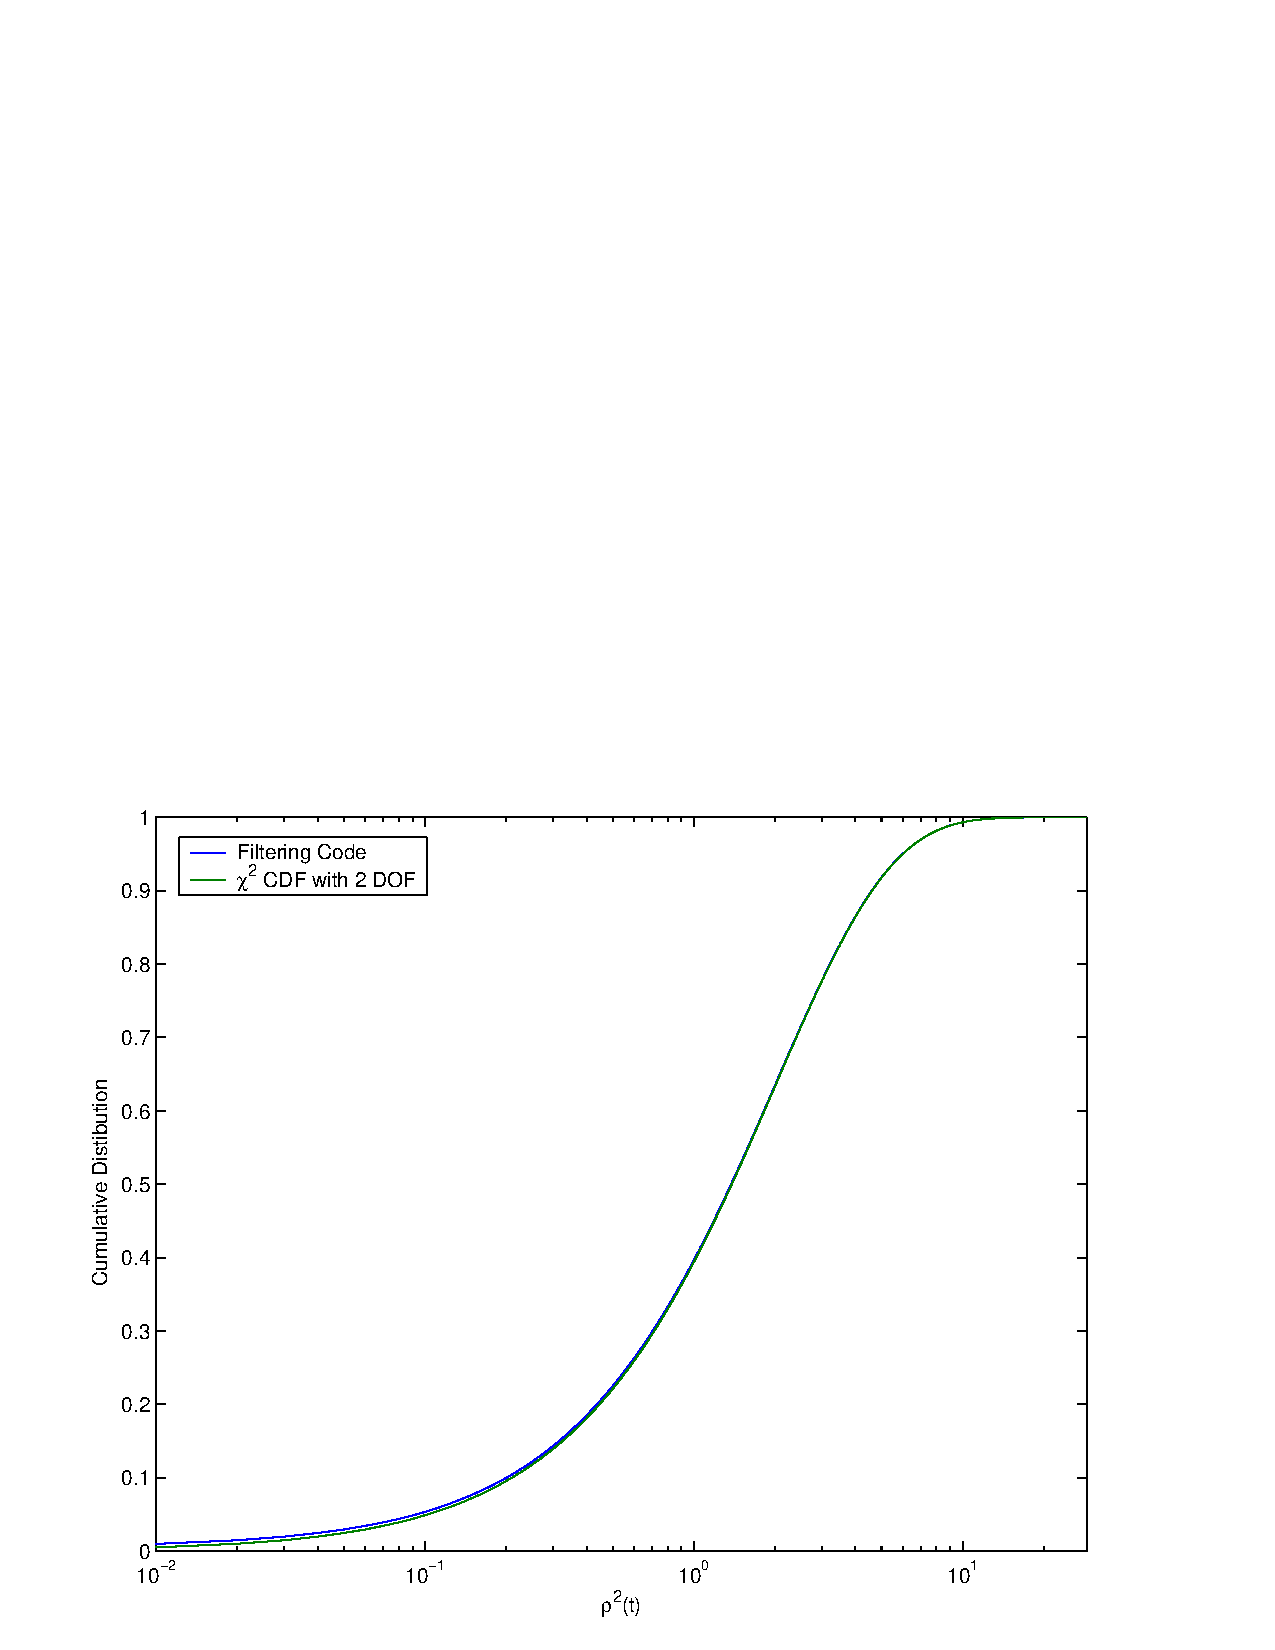
\includegraphics[width=\linewidth]{figures/findchirp/rhosq_gaussian_cdf}
\end{center}
\caption[Distribution of the Filter Output for Gaussian Noise]{%
In the presence of Gaussian noise the expected filter output, $\rho^2(t)$, is
the sum of the squares of two Gaussian distributed quantities and so should be
$\chi^2$ distributed with two degrees of freedom. This figure shows the
cumulative distribution function (CDF) of the filtering code output and the
expected analytic value. The filter input is white Gaussian noise of variance
$\varsigma^2$ and a constant power spectral density of $\ospsd = 2\varsigma^2\delta T$. It
can be seen that there is good agreement between the observed and expected
values.
}
\end{figure}

\begin{figure}[p]
\label{f:impulse_snr}
\begin{center}
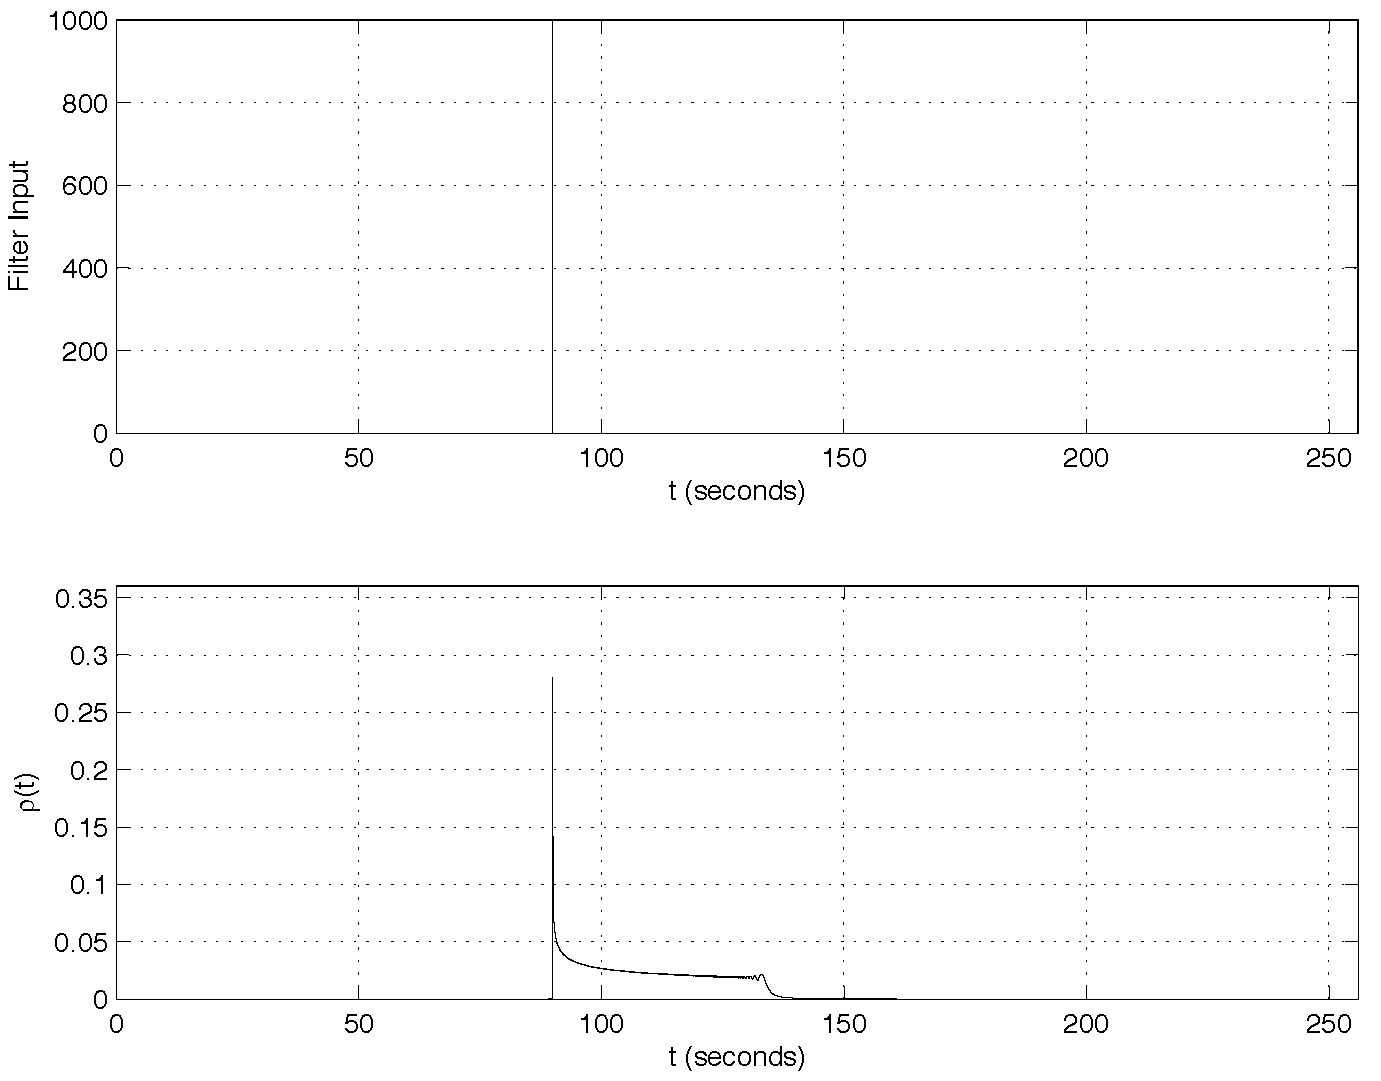
\includegraphics[width=\linewidth]{figures/findchirp/impulse_snr}
\end{center}
\caption[Impulse Response of Matched Filter With a Constant Power Spectrum]{
The top panel shows the filter input which consists of an impulse at $t_0 = 90$.
The power spectrum is set to that of white uncorrelated noise. The bottom panel
shows the output of the filter. The filter output is the sum of the squares of
the time reverse chirps and the maximum of the filter output occurs at the
time of the impulse.
}
\end{figure}

\begin{figure}[p]
\label{f:impulse_spec}
\begin{center}
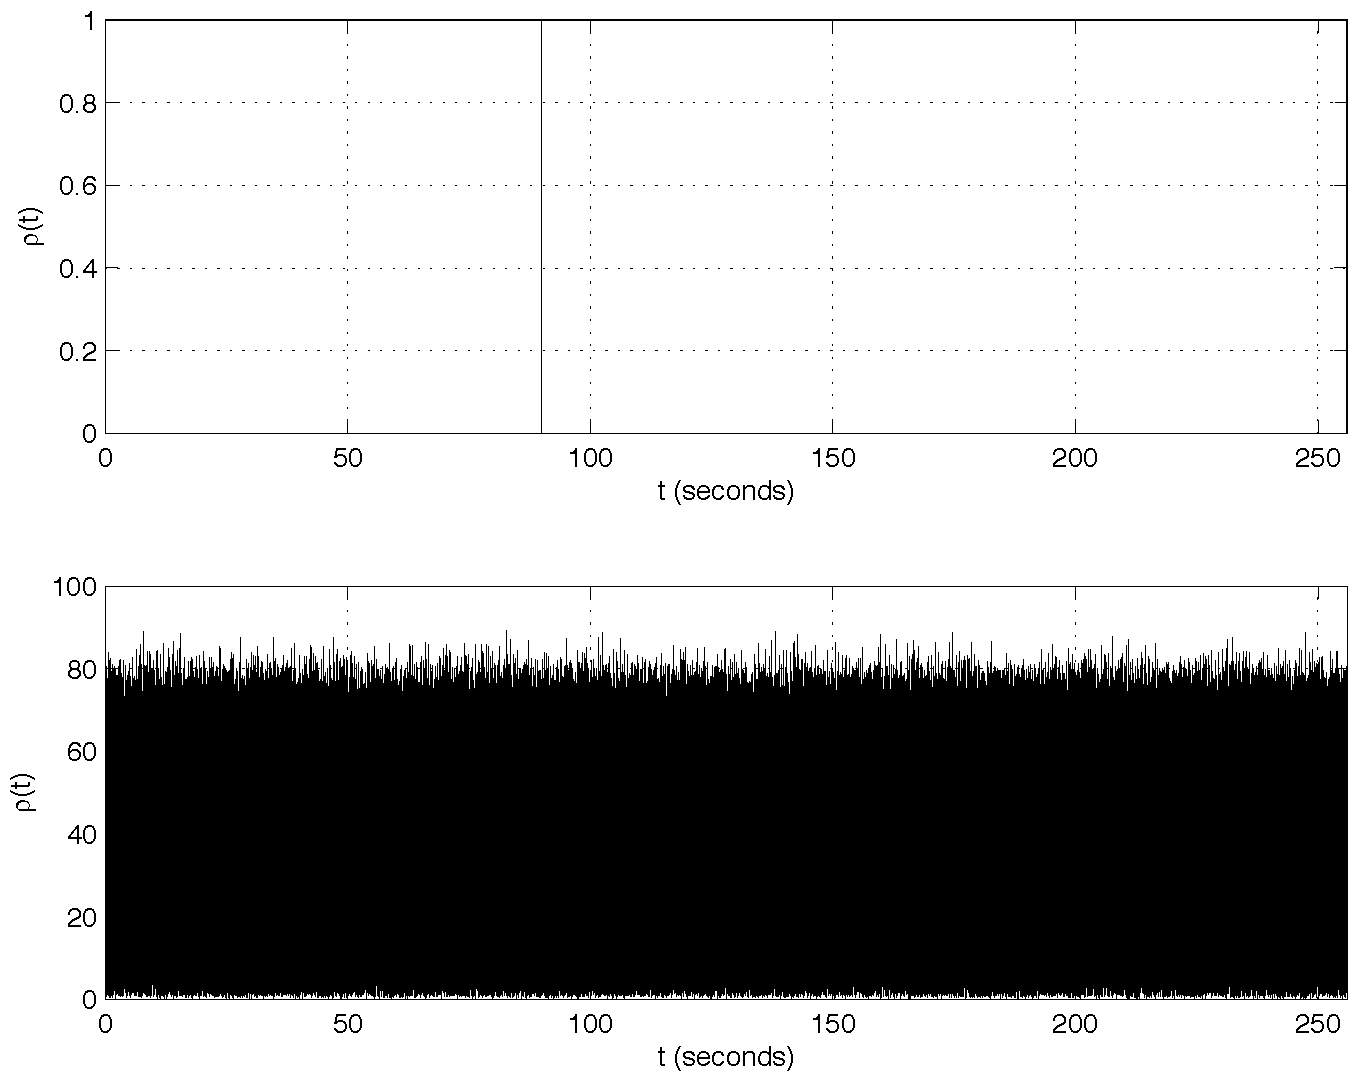
\includegraphics[width=\linewidth]{figures/findchirp/impulse_spec}
\end{center}
\caption[Impulse Response of Matched Filter With a Real Power Spectrum]{
The top panel shows the filter input which consists of an impulse at $t_0 =
90$.  The power spectrum is computed from Gaussian noise of the same length of
the input data using Welch's method. The bottom panel shows the output of the
filter. Due to the fact that the duration of the inverse power spectrum
$1/\ospsd$ in the time domain is the same length as the data segment, the
entire filter output is corrupted due to the wrap around of the FFT.
}
\end{figure}

\begin{figure}[p]
\label{f:impulse_wraparound}
\begin{center}
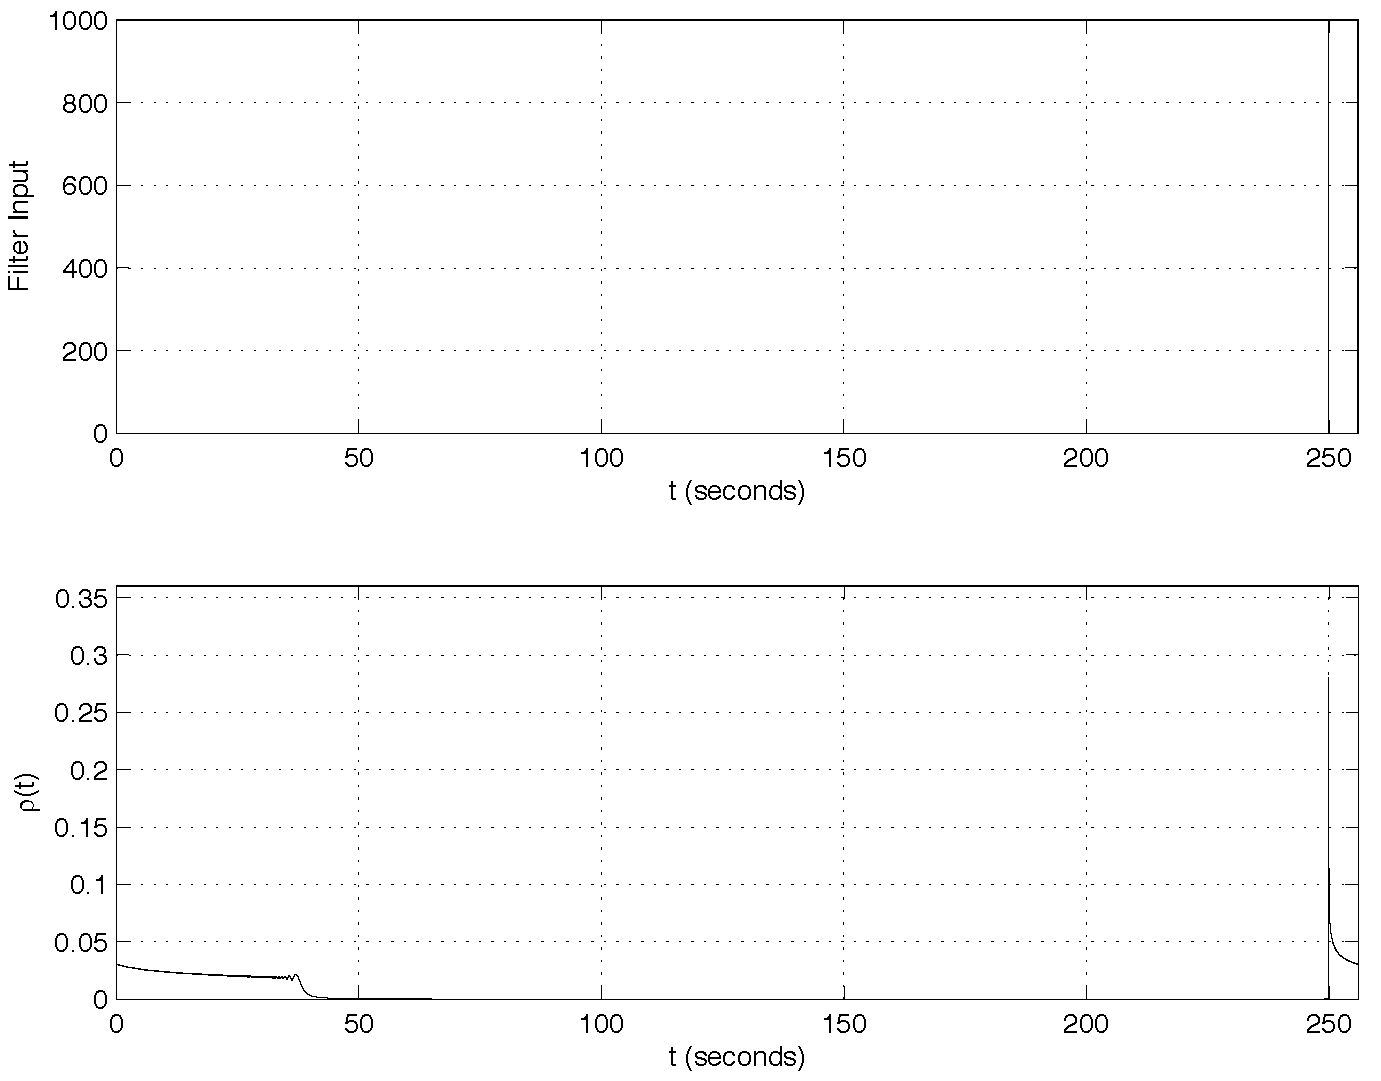
\includegraphics[width=\linewidth]{figures/findchirp/impulse_wraparound}
\end{center}
\caption[Wrap-around of the Matched Filter]{%
The top panel shows the filter input which consists of an impulse at $t_0 = 250$.
The power spectrum is set to that of white uncorrelated noise. The bottom panel
shows the output of the filter. The length of the chirp template is $43.7$
seconds. Notice that the filter output is non-zero for the first $37.7$
seconds of the output due to the wrap-around of the FFT.
}
\end{figure}

\begin{figure}[p]
\label{f:rhosq_median_cdf}
\begin{center}
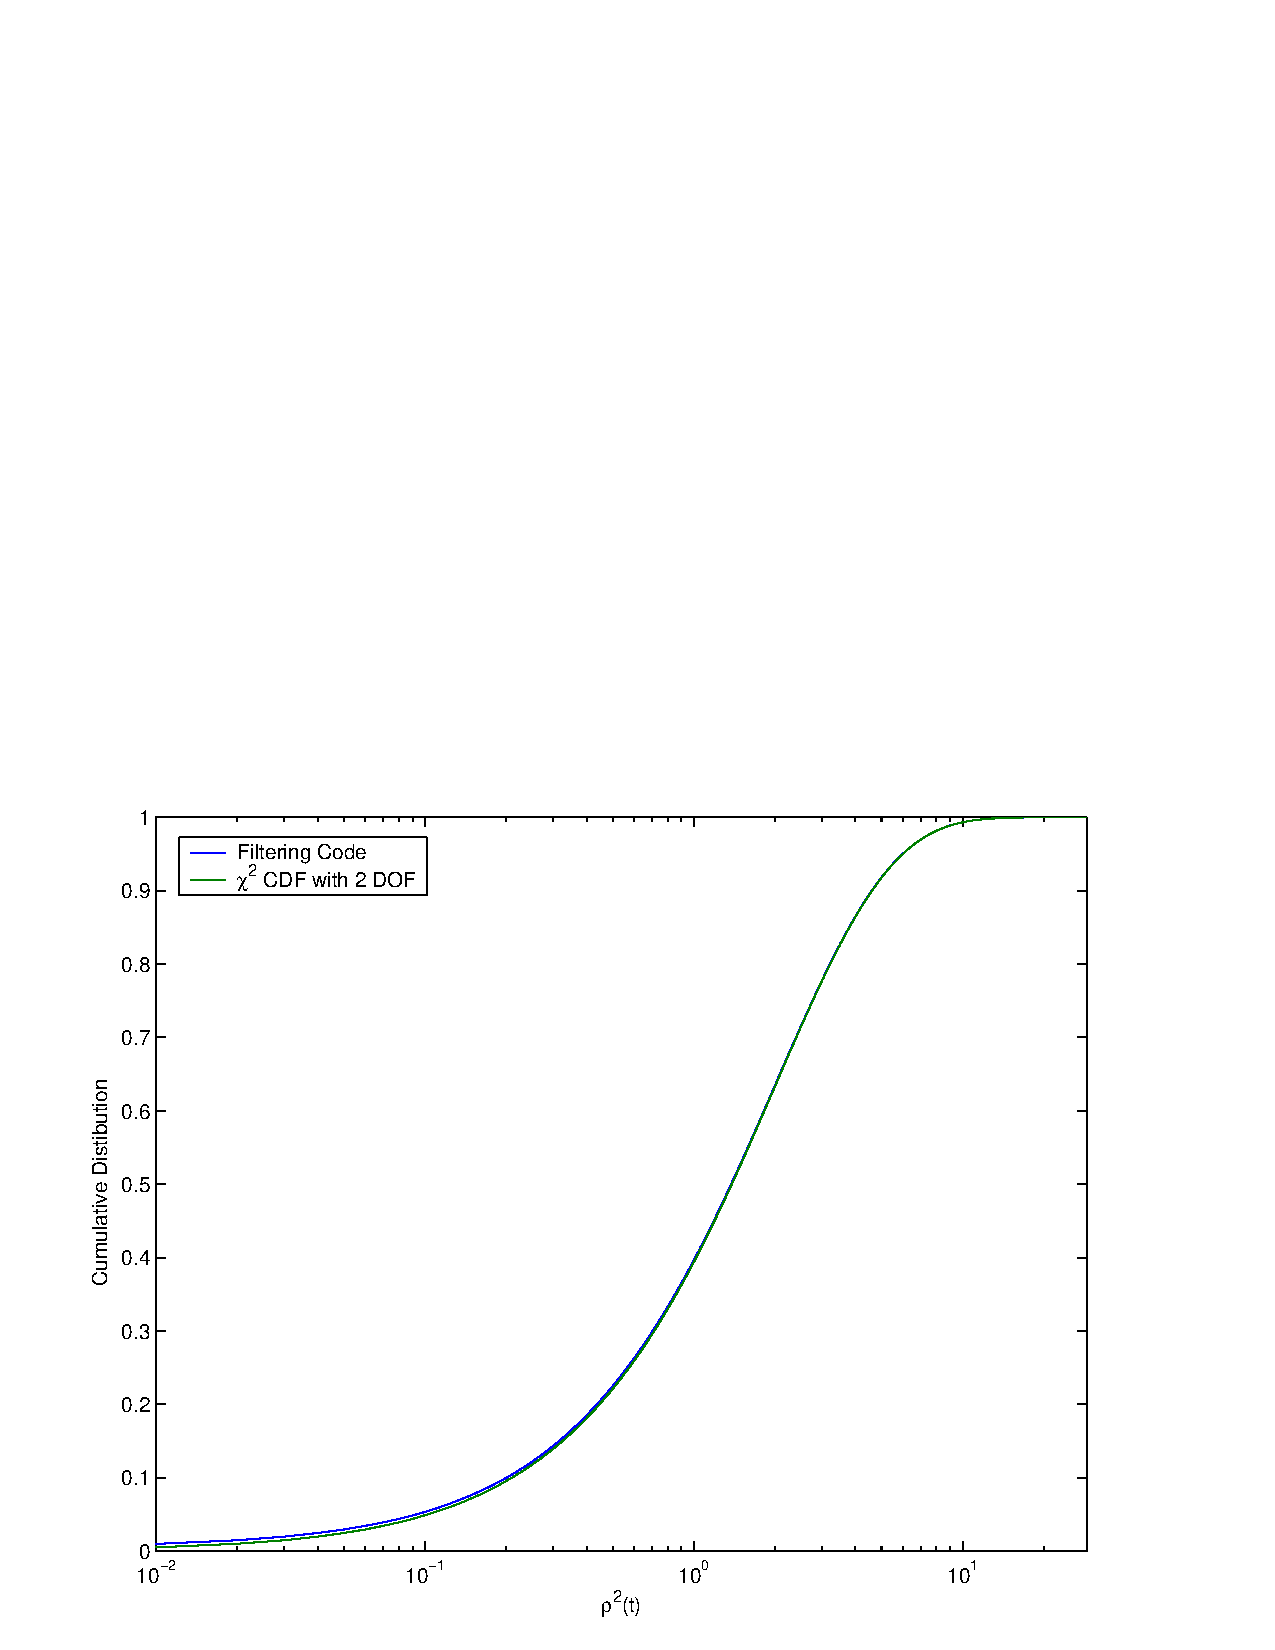
\includegraphics[width=\linewidth]{figures/findchirp/rhosq_gaussian_cdf}
\end{center}
\caption[Distribution of Filter Output Using Median Power Spectral Estimator]{%
In the presence of Gaussian noise the expected filter output, $\rho^2(t)$, is
the sum of the squares of two Gaussian distributed quantities and so should be
$\chi^2$ distributed with two degrees of freedom. This figure shows the
cumulative distribution function (CDF) of the filtering code output and the
expected analytic value. The filter input is white Gaussian noise of length
$256$ seconds and the power spectrum $\ospsd$ is computed from $15$ segments
of white Gaussian noise length $256$ seconds, overlapped by $128$ seconds
using Hann windowing and the median estimator.
}
\end{figure}

\begin{figure}[p]
\label{f:impulse_inv_spec}
\begin{center}
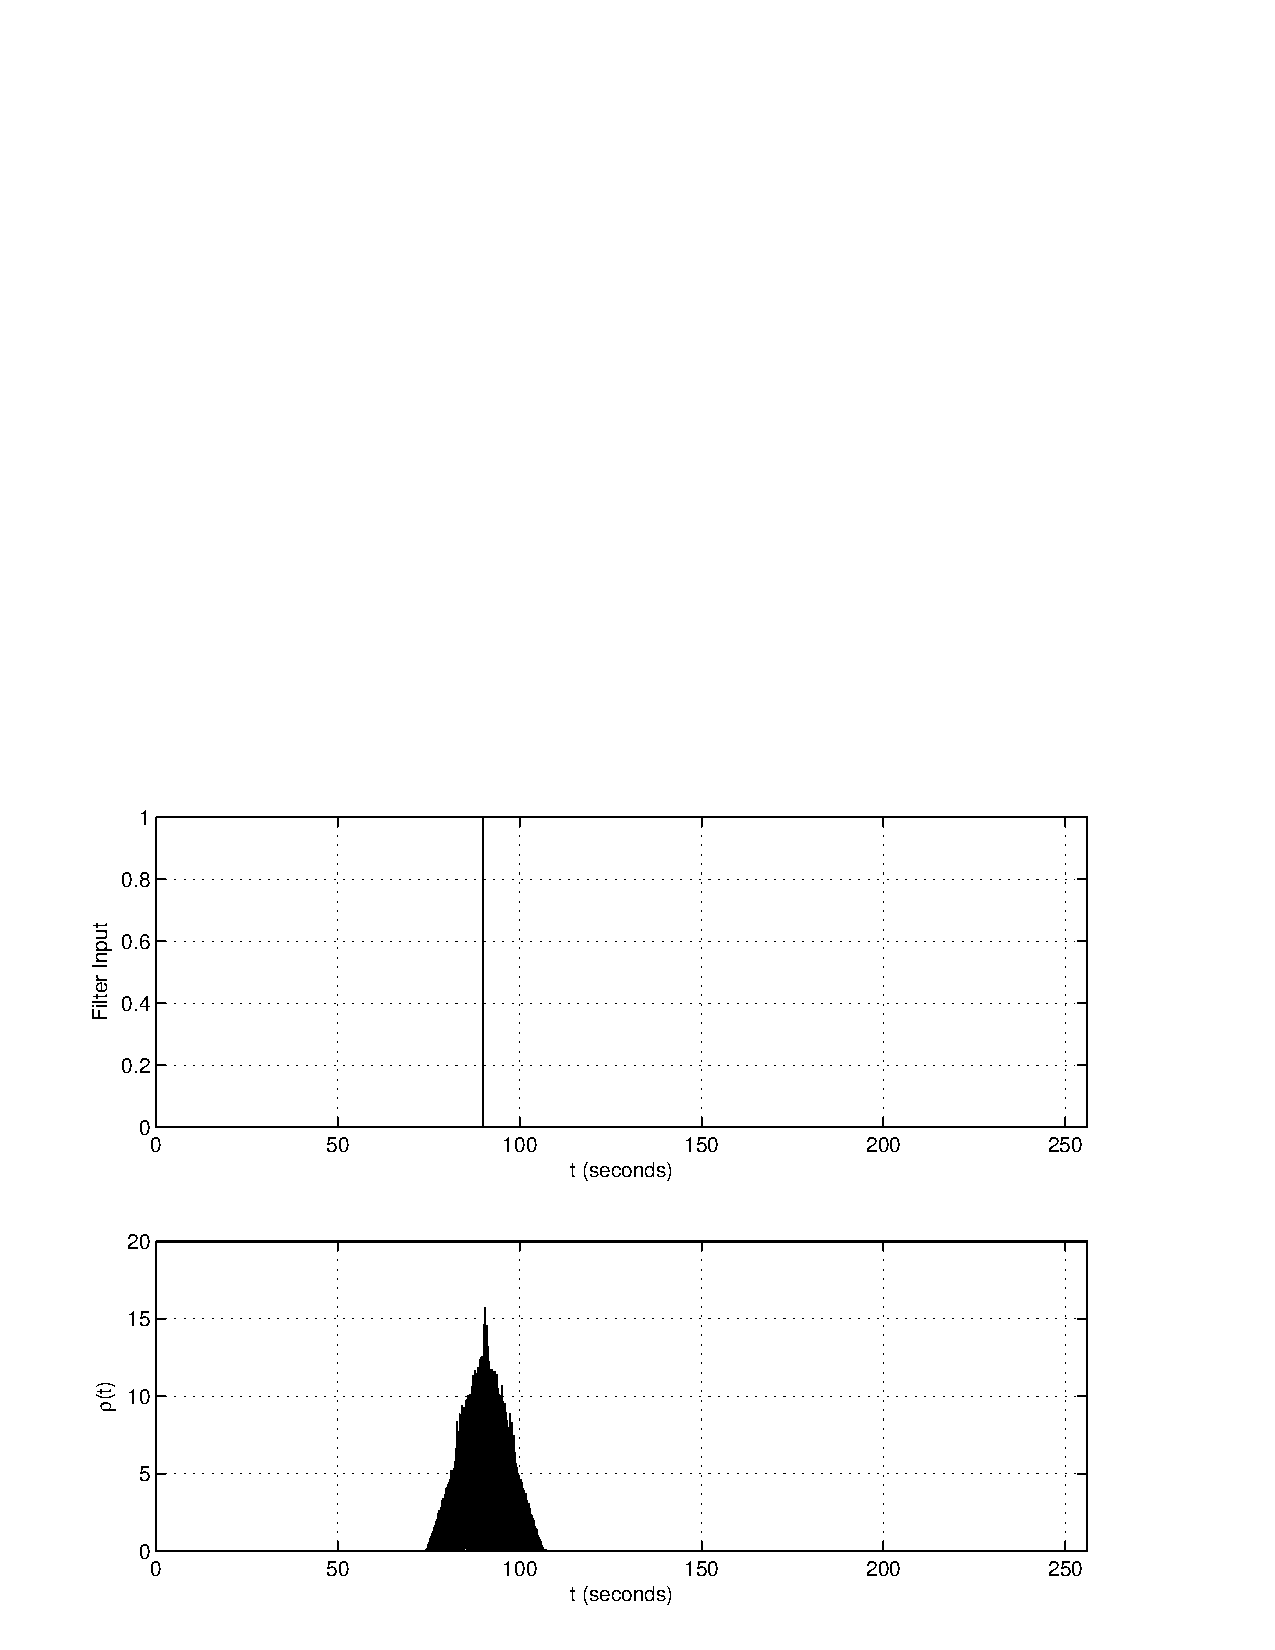
\includegraphics[width=\linewidth]{figures/findchirp/impulse_inv_spec}
\end{center}
\caption[Impulse Response of Matched Filter With a Truncated Power Spectrum]{%
The top panel shows the input to the filtering code which is an impulse at $t
= 90$ seconds. The average power spectrum is computed from typical LIGO noise
and then truncated to $16$ seconds in the time domain. The duration of non-zero
filter output is also $16$ seconds.
}
\end{figure}

\begin{figure}[p]
\label{f:zero_inject_zoom}
\begin{center}
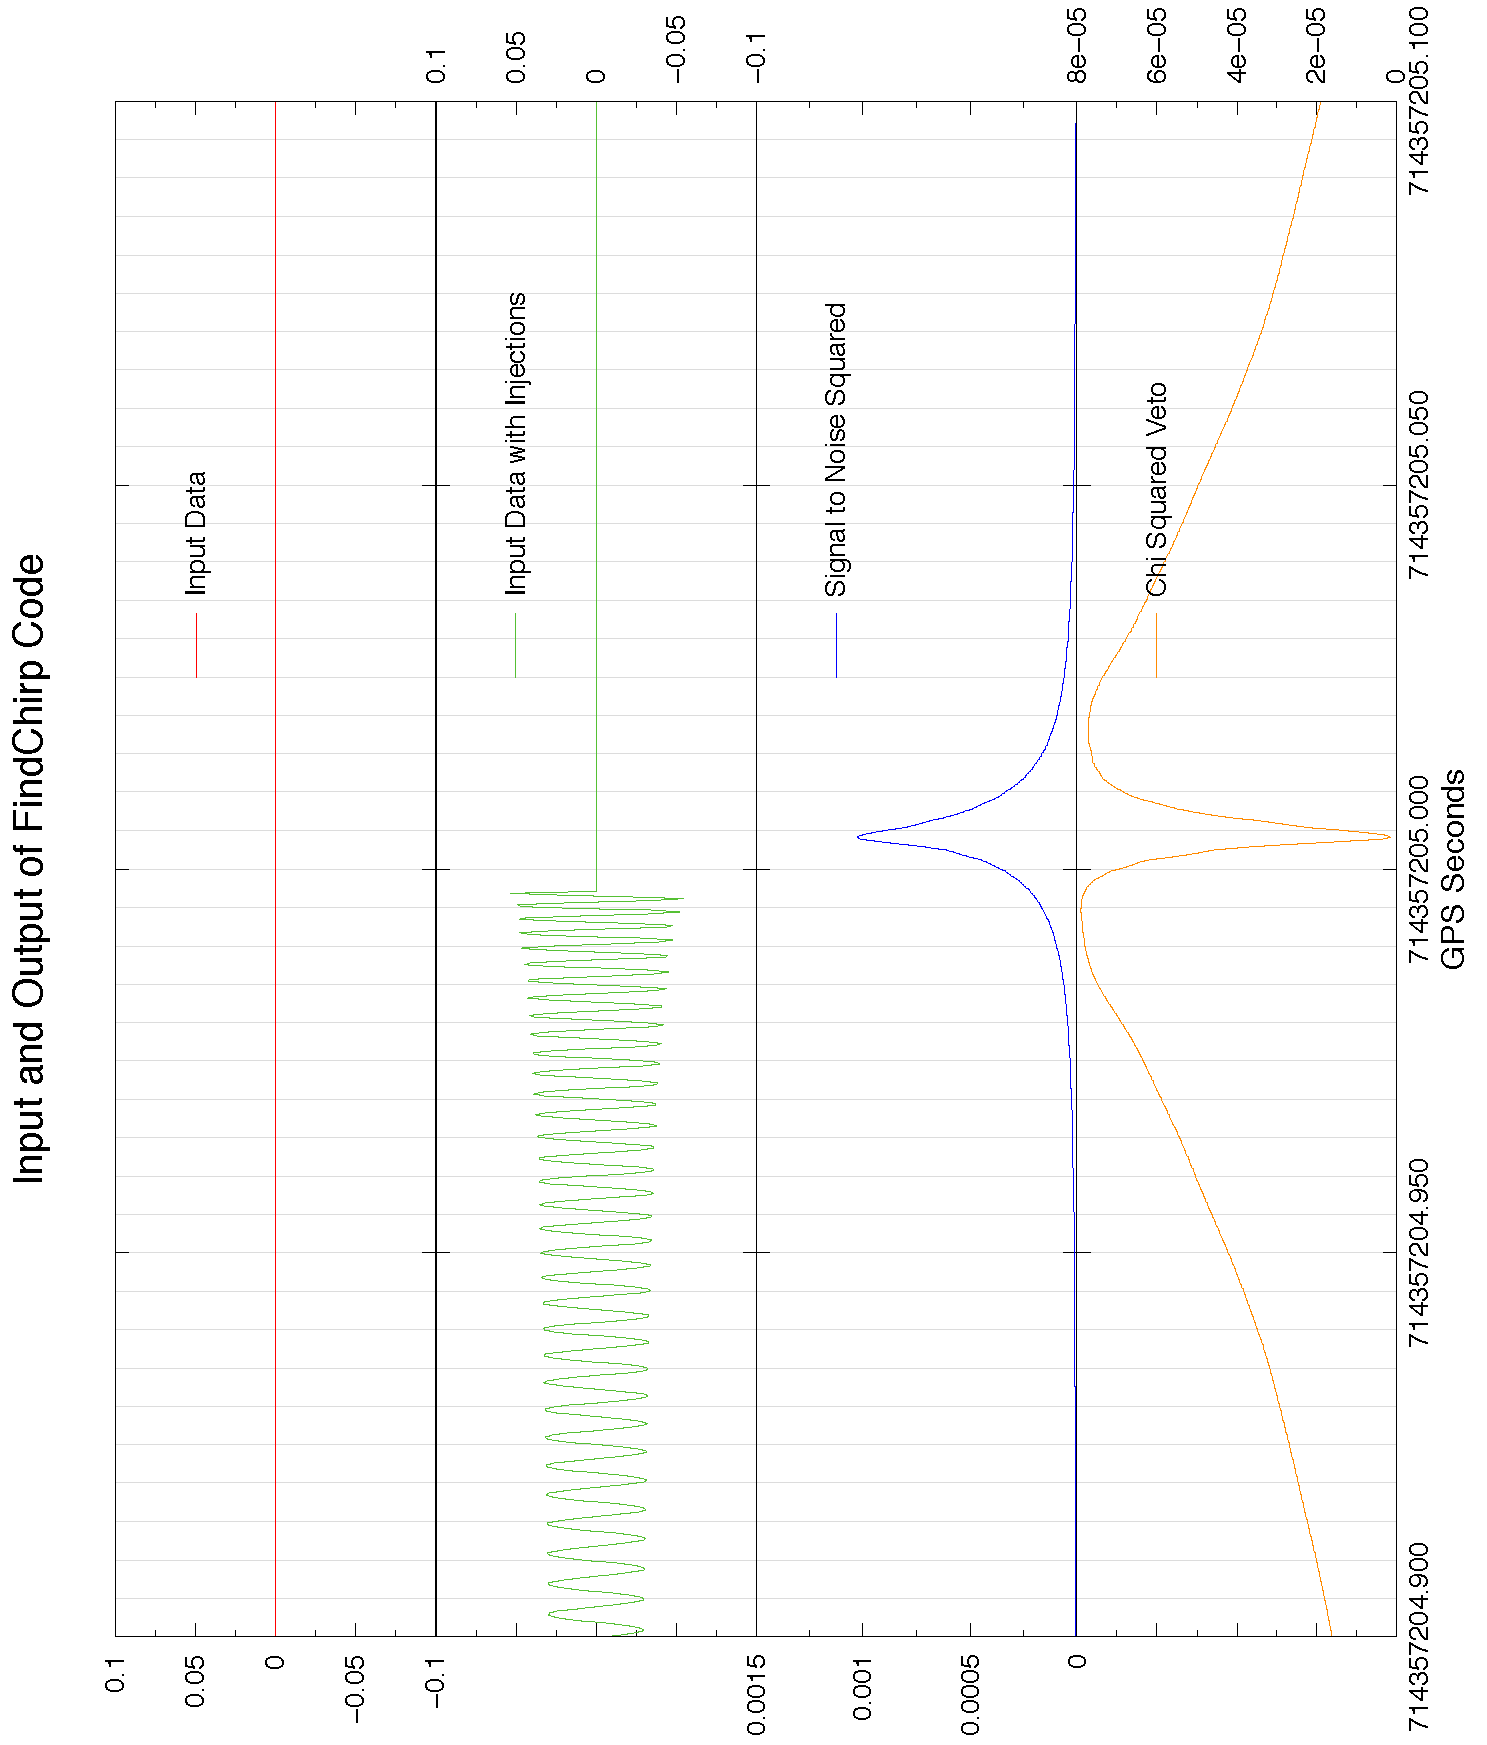
\includegraphics[angle=-90,width=\linewidth]{figures/findchirp/zero_inject_zoom}
\end{center}
\caption[Output of the Filtering Code for a Chirp In the Absence of Noise]{
Output time series from the filtering code
for an inspiral chirp in the absence of noise. A $(2.0,2.0)\,m_\odot$ inspiral
chirp is generated using the post$^2$-Newtonian time domain waveform
generation and injected into the data. This is filtered using the
post$^2$-Newtonian stationary phase waveform. The signal to noise squared and
$\chi^2$ time series are shown.  The signal to noise squared is a maximum at
the coalescence time of the \textit{template} inspiral signal. This occurs
slightly after the coalescence time of the injected signal. The difference in
coalescence times is due to the different methods of generating the chirp
signal.
}
\end{figure}

\begin{figure}[p]
\label{f:maxoverchirp}
\begin{center}
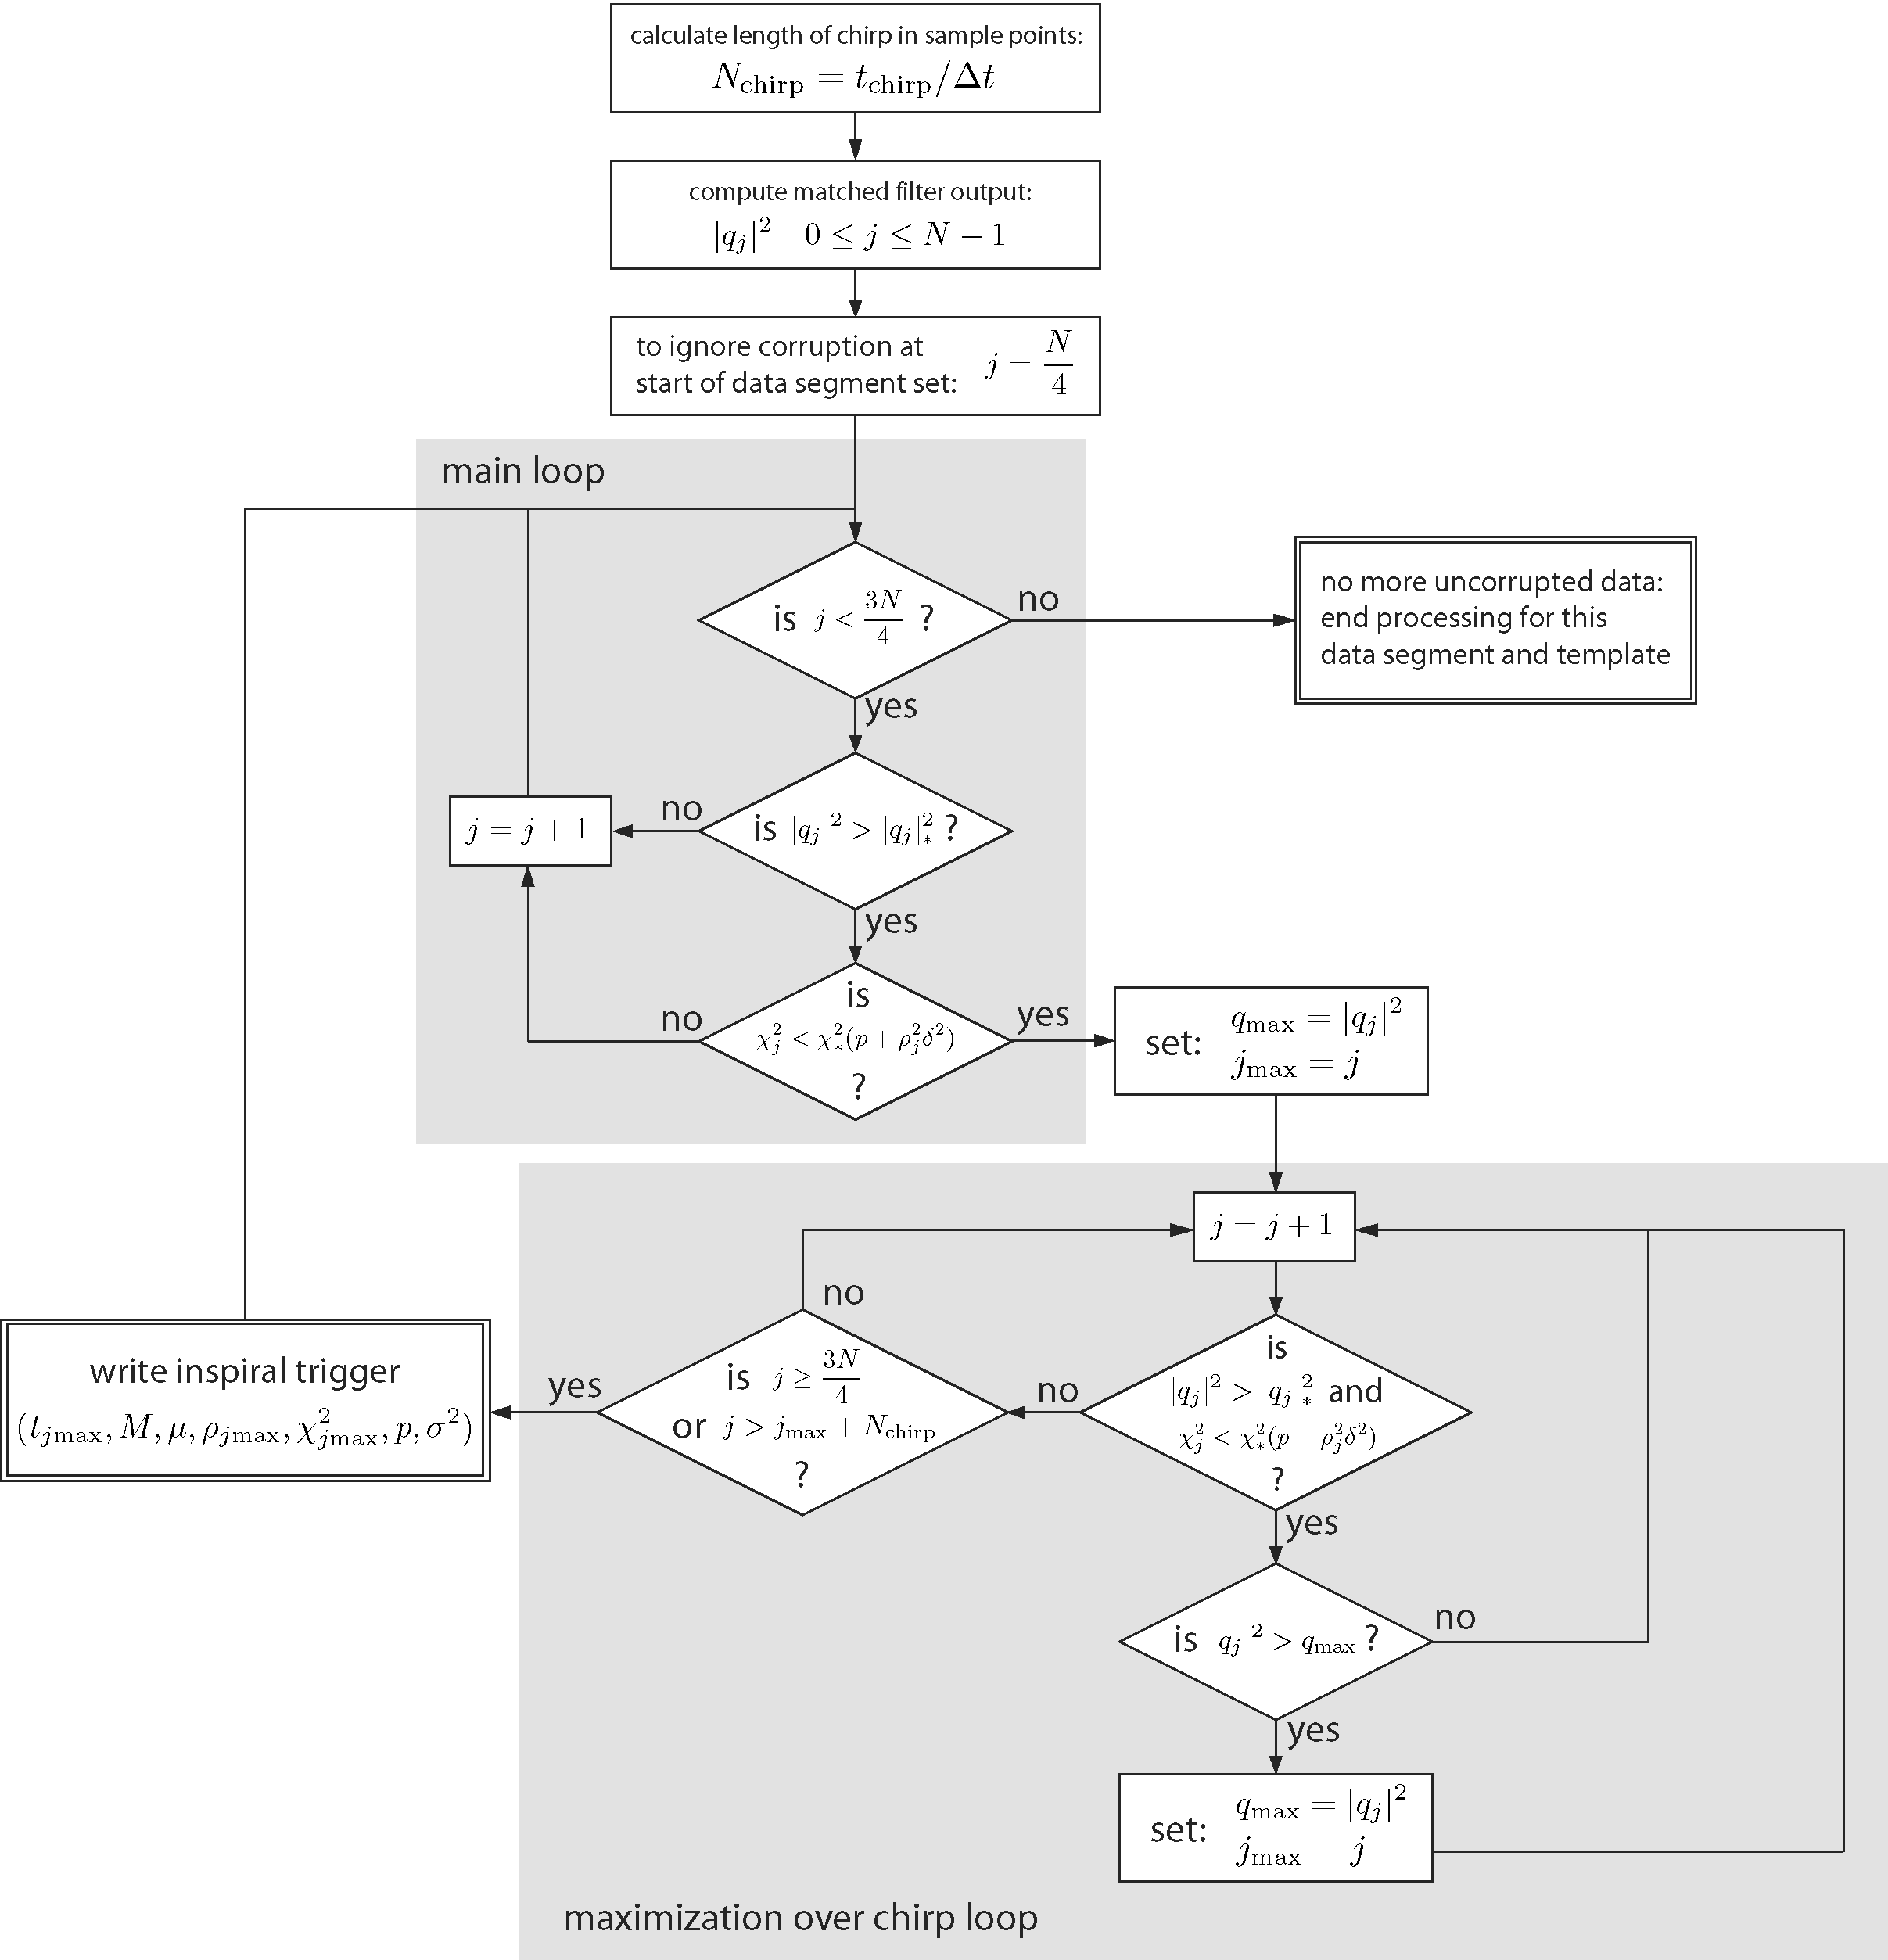
\includegraphics[width=\linewidth]{figures/findchirp/maxoverchirp}
\end{center}
\caption[Inspiral Trigger Selection Algorithm]{
The algorithm used to generate inspiral triggers. For a given inspiral
template we begin by calculating the length of the chirp and the filter
output. For a data segment of length $N$, the first and last $N/4$ points in
the segment may be corrupted due to FFT wrap-around, so we ignore them. For
the rest of the data segment, we step through the filter output looking for
times when the signal-to-noise and $\chi^2$ threshold are satisfied (the main
loop). If we find a point that passes the threshold tests, we label it
$j_\mathrm{max}$ and enter the maximization over chirp loop. This steps
through the data looking for the any larger values of $|q_j|^2$ within a chirp
length (given by $N_\mathrm{chirp}$) of the time $j_\mathrm{max}$. If a larger
value of $|q_j|^2$ is found, we reset $j_\mathrm{max}$ and keep looking for
any larger values. If no larger value is found within a chirp length (or we
reach the end of the uncorrupted data) we generate an inspiral trigger and
save its time, mass, signal-to-noise ratio, value of the $\chi^2$ veto, number
of $\chi^2$ bin ($p$) and the value of $\sigma^2$ for this data segment. 
}
\end{figure}

